%# -*- coding: utf-8-unix -*-
%%==================================================
%% thesis.tex
%%==================================================

% 双面打印
\documentclass[master, fontset=adobe, openright, twoside, zihao=-4]{sjtuthesis}
% \documentclass[bachelor, fontset=adobe, openany, oneside, zihao=-4, submit]{sjtuthesis} 
% \documentclass[master, adobefonts, review]{sjtuthesis} 
% \documentclass[%
%   bachelor|master|doctor,	% 必选项
%   fontset=adobe|windows,  	% 只测试了adobe
%   oneside|twoside,		% 单面打印,双面打印(奇偶页交换页边距,默认)
%   openany|openright, 		% 可以在奇数或者偶数页开新章|只在奇数页开新章(默认)
%   zihao=-4|5,, 		% 正文字号:小四、五号(默认)
%   review,	 		% 盲审论文,隐去作者姓名、学号、导师姓名、致谢、发表论文和参与的项目
%   submit			% 定稿提交的论文,插入签名扫描版的原创性声明、授权声明 
% ]

% 逐个导入参考文献数据库
\usepackage{caption,setspace}
\usepackage{graphics}
\usepackage{graphicx}
\usepackage{multirow}
\usepackage{bm}
\usepackage{biblatex}
\usepackage{subfigure}
\usepackage{algorithm}
\usepackage{algorithmic}
\usepackage{amsmath}

%\addbibresource{bib/thesis.bib}
% \addbibresource{bib/chap2.bib}



%\bibliography{bib/thesis}

\begin{document}

%% 无编号内容:中英文论文封面、授权页
%# -*- coding: utf-8-unix -*-
\title{基于一致性特征的非交互式差分隐私优化算法}
\author{钱\quad{}磊}
\advisor{梁阿磊副教授}
% \coadvisor{某某教授}
\defenddate{2014年12月17日}
\school{上海交通大学}
\institute{软件工程}
\studentnumber{1130379037}
\major{软件工程}

\englishtitle{Optimizing the Range-Count Queries in Differential Privacy}
\englishauthor{\textsc{Lei Qian}}
\englishadvisor{Prof. \textsc{Alei Liang}}
% \englishcoadvisor{Prof. \textsc{Uom Uom}}
\englishschool{Shanghai Jiao Tong University}
\englishinstitute{\textsc{School of Software Engineering} \\
  \textsc{Shanghai Jiao Tong University} \\
  \textsc{Shanghai, P.R.China}}
\englishmajor{Software Engineering}
\englishdate{Dec. 17th, 2015}


\maketitle

\makeenglishtitle

\makeatletter
\ifsjtu@submit\relax
	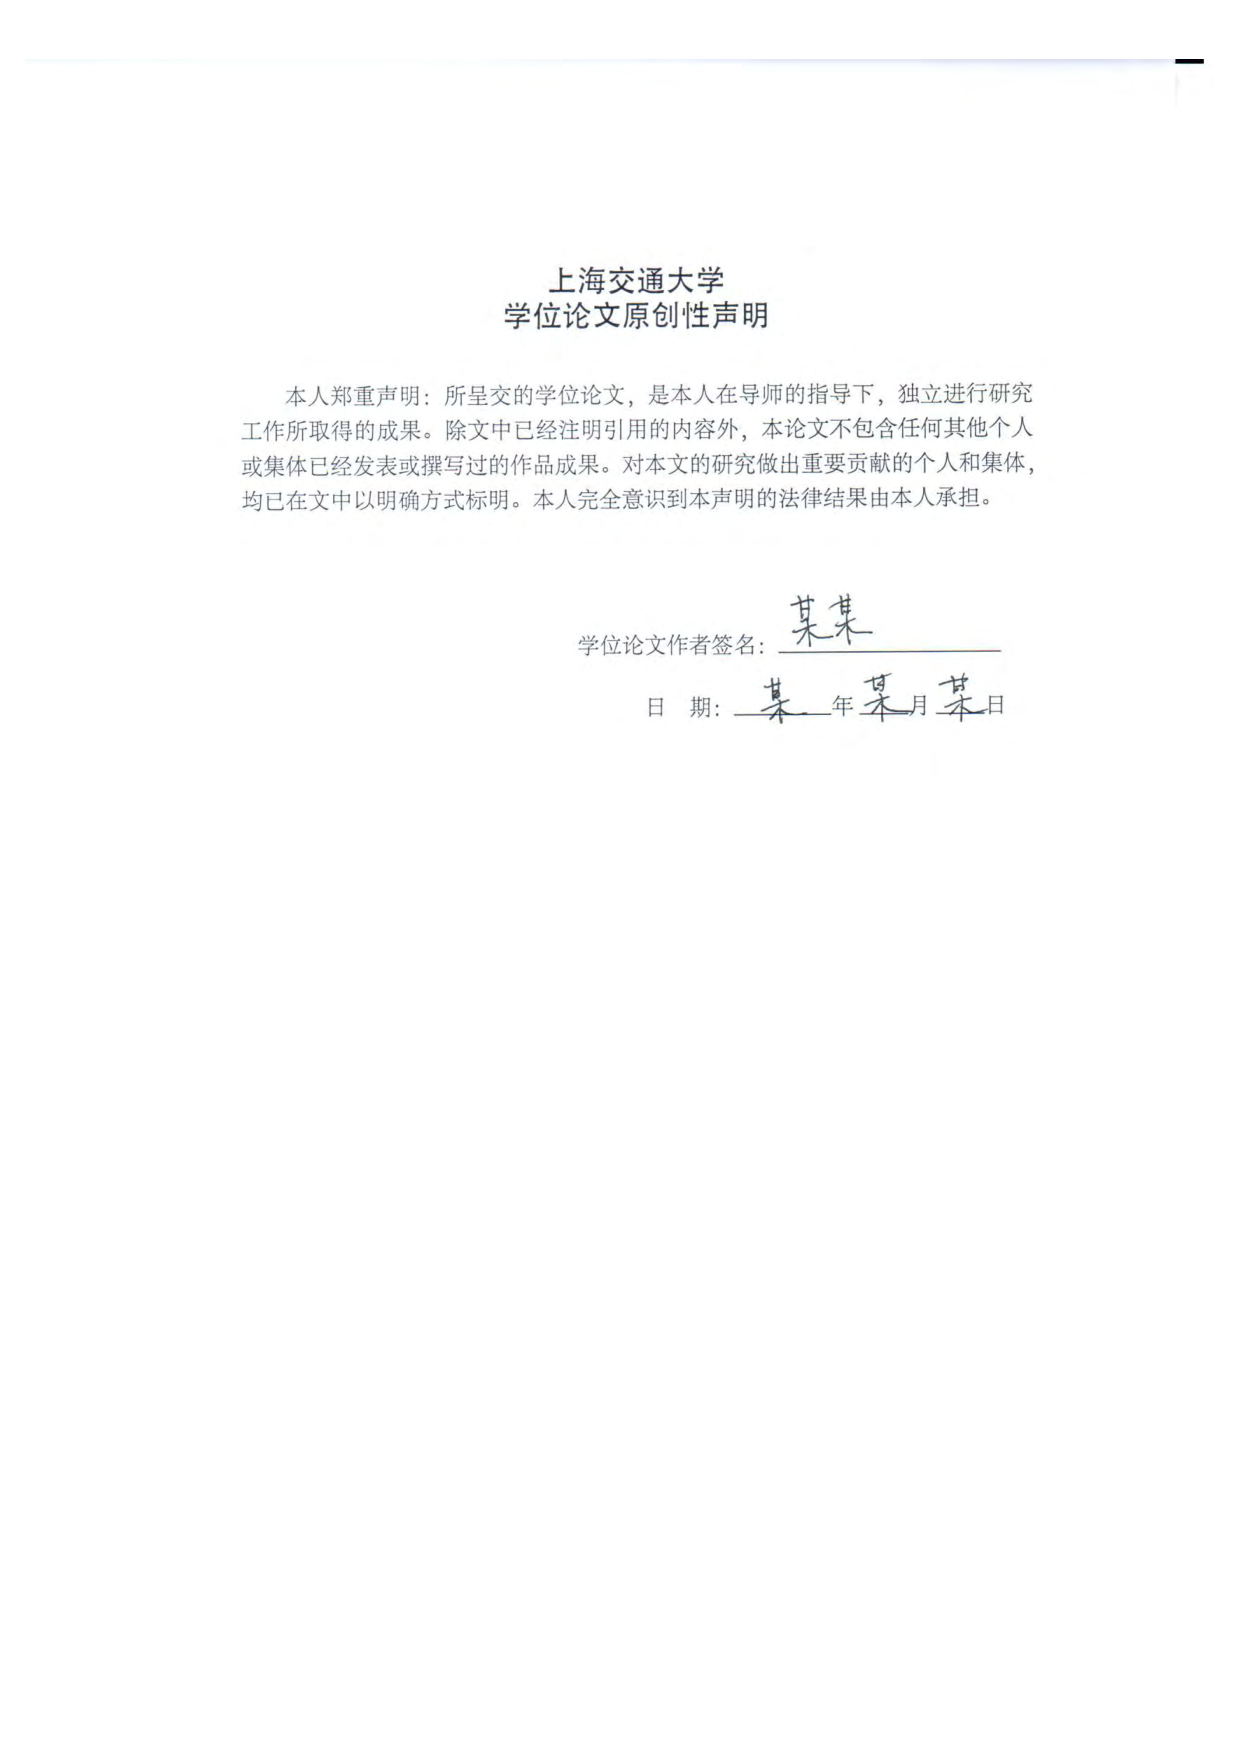
\includepdf{pdf/original.pdf}
	\cleardoublepage
	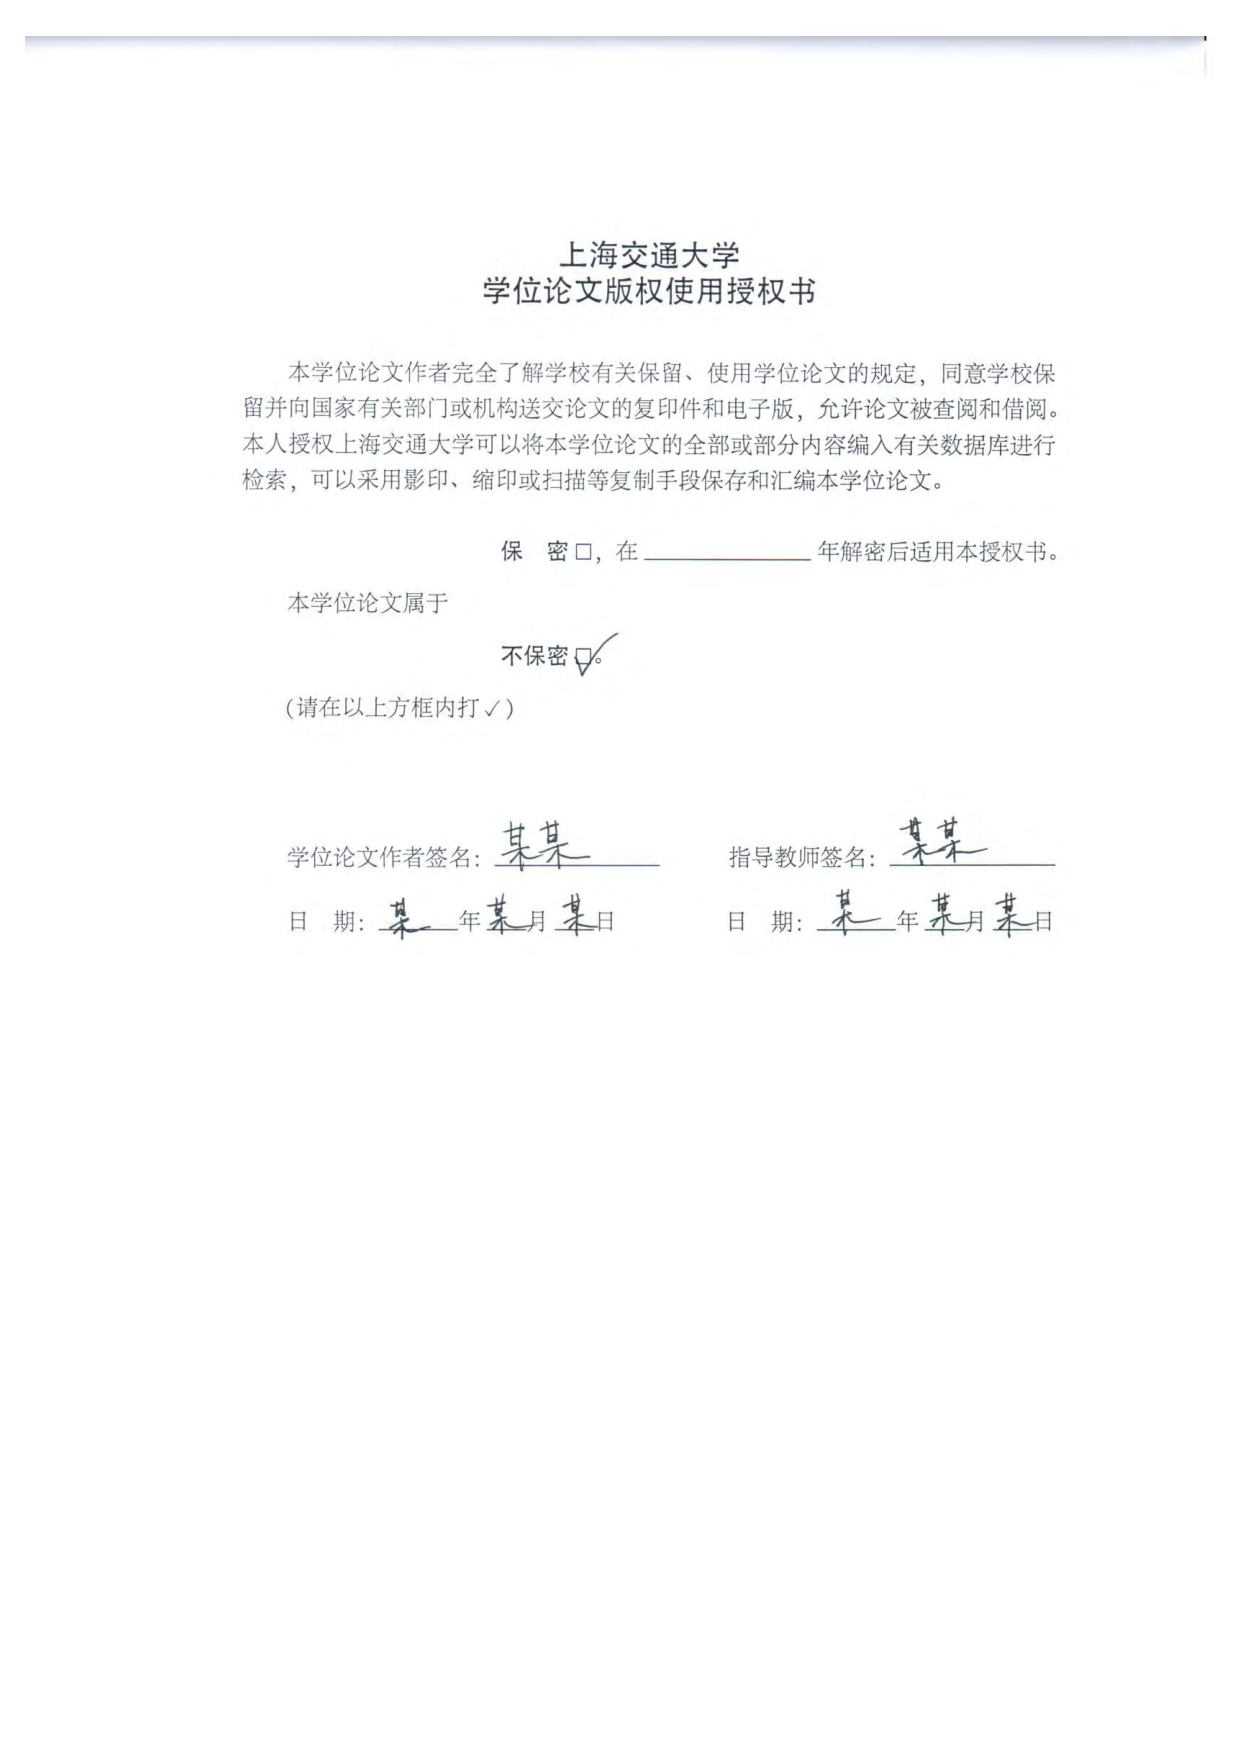
\includepdf{pdf/authorization.pdf}
	\cleardoublepage
\else
	\makeDeclareOriginal
	\makeDeclareAuthorization
\fi
\makeatother


\frontmatter 	% 使用罗马数字对前言编号

%% 摘要
\pagestyle{main}
%# -*- coding: utf-8-unix -*-
%%==================================================
%% abstract.tex for SJTU Master Thesis
%%==================================================

\begin{abstract}

高速发展的数据应用技术让数据的潜在价值得到了充分的利用,但是新的数据挖掘模式和攻击手段的出现使得传统的隐私保护方式变得不那么安全可靠了。一方面,数据拥有者在发布数据时需要对隐私信息进行特殊处理;另一方面,发布后的数据可能会应用于各类数据挖掘算法,此时也应该保障隐私安全。对数据拥有者而言,面对各种无法预计的攻击及数据挖掘模式,如何设计具有强力隐私保障的隐私保护算法成了难点问题。

针对上述情况,直到差分隐私技术的出现才从根本上解决这个问题。它不关心具体的应用背景,即使在最坏的情况下攻击者已经掌握了除了某条记录之外的所有记录信息,也无法推断出该条记录的隐私信息情况。但基于失真技术的加噪操作会使得差分隐私技术在保护隐私的同时影响了数据的可用性,降低了后续应用的分类准确度,这就对差分隐私算法的设计提出了新的要求。

本文基于差分隐私技术在数据挖掘分类算法中的应用,就查询维度引起的噪音叠加问题,设计一种利用数据一致性特性对噪音分布进行优化的非交互式差分隐私算法DiffCon,使得在保障数据隐私的前提下,有效提升发布数据在高维度查询应用中的可用性。

本文的主要工作包括:1)分析现有的基于决策树构造方式的差分隐私匿名算法,总结高维度查询产生的维度灾难问题成为影响算法可用性的关键因素。2)研究此算法与后续的数据挖掘分类算法间的联系,概括其本质模型。%查询维度相关的噪音叠加现象制约了算法扩展性的提升。
3)基于重匿名属性值间的一致性特性,设计并实现DiffCon,达到提升发布数据分类准确度的目的。


%现在各种数据面临的问题:1,发布的数据要不能泄露隐私。2,经得起各种数据挖掘分析。
%关注点:1,如何满足差分隐私。2,发布出的数据可用性的保障。
%厉害之处:保 护 方 法 可 以 确保 在 某 一 数 据 集 中 插 入 或 者 删 除 一 条 记 录 的 操 作不 会 影 响 任 何 计 算 的 输 出 结 果 另 外该 保 护 模 型不关心攻击者所具有的背景知识即 使 攻 击 者 已经掌握除某一条记录之外的所有记录的信息 该记 录 的 隐 私 也 无 法 被 披 露 
%两种数据保护框架:交互式和非交互式
%关键字:决策树,k匿名
%1,决策树的基本用法,fireman,然后匿名化得diffGen。 维度问题:主要指查询维度,从而有噪音叠加问题。 指出构造树和后续的决策树计数应用之间的联系。提出一致性

\keywords{\large 隐私保护 \quad 差分隐私 \quad 决策树 \quad 匿名化 \quad 一致性}
\end{abstract}

\begin{englishabstract}

fdfdfsdfsfdsfsdfsdfdsfsdfsdf

\englishkeywords{\large SJTU, master thesis, XeTeX/LaTeX template}
\end{englishabstract}



%% 目录、插图目录、表格目录
\tableofcontents
\listoffigures
\addcontentsline{toc}{chapter}{\listfigurename} %将插图目录加入全文目录
\listoftables
\addcontentsline{toc}{chapter}{\listtablename}  %将表格目录加入全文目录
% \listofalgorithms
% \addcontentsline{toc}{chapter}{代码索引}  %将表格目录加入全文目录

%# -*- coding: utf-8-unix -*-
\chapter{主要符号对照表}
\label{chap:symb}

\begin{longtable}{rl}
$\epsilon$     & 隐私代价 \\
$DP$ 		& 差分隐私(Differential Privacy) \\

\end{longtable}
 % 主要符号、缩略词对照表

\mainmatter	% 使用阿拉伯数字对正文编号

%% 正文内容
\pagestyle{main}
%# -*- coding: utf-8-unix -*-
%%==================================================
%% chapter01.tex for SJTU Master Thesis
%%==================================================

\chapter{绪论}
\label{chap:introduction}

\section{引言}
\label{sec:objective}
隐私是一种与公共、群体利益无关,不便或者不愿他人知道的、应予以保密的信息,是不以他人是否承认或评价为转移的存在。从人类有意识开始,隐私意识便是最先表现出来的本能特征,伴随着时代文明的发展,人类具有越来越强的隐私保护意识。“数据时代”的飞速发展使得信息数据的采集、存储和发布变得更加方便快捷,海量数据的处理技术以及数据挖掘、机器学习算法的应用使得数据的共享和分析变得更加高效准确,与此同时新的隐私攻击手段,黑客技术也在不断涌现。可见科技和时代的发展在带给我们高品质生活的同时,数据中的隐私保护问题面临着愈加严峻的挑战。
本课题基于最高隐私保障的差分隐私技术,通过设计对高纬度查询问题具有良好扩展性的非交互式差分隐私匿名算法,有效提升了发布数据在后续数据挖掘分类算法中的分类准确度。本章节将简要介绍相关的课题背景知识,总结各类隐私保护算法和面向数据挖掘分类问题的研究现状,最后明确研究目标和所要解决的问题。


\section{课题研究背景}

\subsection{隐私及隐私保护}  %隐私的定义,度量,泄露风险及隐私保护研究方向

隐私指的是个体不愿被外界获悉的敏感属性,比如个人的病理特征,资产状况,家庭住址等。隐私分为两类\cite{Defining Privacy for Data}:(1)个人隐私(individual privacy):任何可以直接或间接标识特定人物且不愿被披露的信息,可以是个人的物理信息,生理信息或社会属性信息等。(2)共同隐私(corporate privacy):包含了所有人共同的个人隐私的信息,如工厂工人的薪资分布。

隐私的保护程度可以用隐私的“披露风险”(disclosure risk)\cite{l-diversity}来度量,披露风险越高意味着隐私保护程度越低。披露风险是与攻击者所具备的背景知识(background knowledge)相关的\cite{面向数据库应用的隐私保护研究综述},若s表示隐私信息,Pr[E]表示事件E发生的概率,那么在公布背景知识E的前提下隐私信息s披露的风险\textsc{R}(s,E)表示为
\[
	\textsc{R}(s,E) = Pr(E_{s}).
\]
披露风险\textsc{R}(s,E)可以用来度量隐私保护程度,如$l$-diversity算法\cite{l-diversity}保证隐私披露风险不超过1/$l$,$m$-Invariance算法\cite{m-Invariance}的披露风险不超过1/$m$。

隐私保护的研究方向是由具体应用领域的需求来决定。面向数据挖掘类应用的隐私保护技术主要是研究针对某类数据挖掘算法,根据其特性设计出适应性良好的隐私保护算法,如Clustering\cite{clustering}算法;基于数据发布的隐私保护技术,主要是通过泛化或加密技术发布处理后的数据提供给各类应用,如一系列匿名化算法\cite{multidimensional k anonymity};面向分布式环境下的隐私保护技术,如在智能电网中的应用\cite{Distributed Privacy}。

隐私保护手段大体上分为4类\cite{面向数据库应用的隐私保护研究综述}:(1)基于数据失真(distorting)的技术,如通过添加噪音(noise)的方式达到模糊敏感数据的目的,同时保持数据集的统计特征。(2)基于数据加密技术隐藏敏感数据。(3)基于限制发布的保护技术,如泛化数据域。(4)结合以上三种方式的优点生成的新方法。


\subsection{差分隐私背景} %交互和非交互框架,隐私代价分配和消耗 列联表 直方图

$\varepsilon$-差分隐私($\varepsilon$-differential privacy)\cite{Dwork Calibrating}不同于传统的隐私保护技术,它对隐私披露风险给出了严谨的量化证明,并且定义了严格的攻击模式,因此不关心攻击者所获取的背景知识。通过拉普拉斯加噪机制\cite{Dwork Calibrating}设计满足差分隐私定义的算法,就能够给数据提供最高级别的隐私保障力度。$\varepsilon$是隐私预算(private budget),表示隐私的保护程度,$\varepsilon$越小则隐私保护程度越高。
差分隐私技术的研究主要在于两个方面:(1)如何设计满足差分隐私定义的隐私保护算法。(2)如何减少噪音扰动,保证加噪后数据的高可用性。

差分隐私保护框架分为两种:交互式框架和非交互式框架,如下图\ref{fig:interactive framework}和图\ref{fig:non-interactive framework}所示。在交互式框架中,用户提交查询请求给数据库之后,数据库的应答作为某种差分隐私处理算法的输入,返回输出结果给用户。这个过程中差分隐私处理算法成为了用户和数据库之间的查询接口,但经过一定数量的查询之后耗尽隐私预算$\varepsilon$,对于之后的查询就无法保证隐私保护质量了,因此不再满足差分隐私定义。
在非交互式框架中,数据库先将包含隐私信息的原数据集交于差分隐私算法处理,接着发布整个处理后数据集给用户,或者采用常规数据库查询模式给予应答。这个离线模式的框架具有诸多优点,并且不存在隐私预算耗尽的问题,更多的研究点在于考虑如何提升发布数据可用性和分析准确度。

\begin{figure}[!htp]
	\centering
	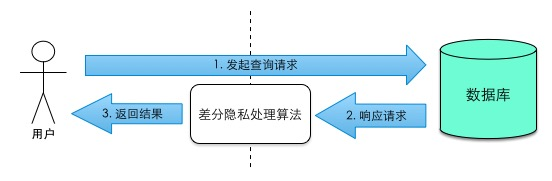
\includegraphics[width=5in]{chap1/interactive}
	\bicaption[fig:interactive framework]{图}{交互式框架}{Fig.}{interactive framework}
\end{figure}

\begin{figure}[!htp]
	\centering
	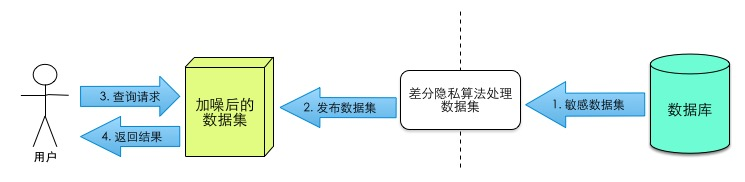
\includegraphics[width=5in]{chap1/non-interactive}
	\bicaption[fig:non-interactive framework]{图}{非交互式框架}{Fig.}{non-interactive framework}
\end{figure}


\subsection{决策树} %主要的数据挖掘分类算法,信息增益,C4.5,CART对于离散和连续属性的处理问题

数据挖掘分类算法是一种监督学习(Supervised Learning)算法,典型代表是决策树模型(Decision Tree)\cite{decision tree},它通过构建树状的分类模型,在每个内部节点做属性选取以及样本分类,最后在叶节点标识类别属性。构建树的过程中属性的选择方式是决策树算法的关键,直接影响到分类性能的好坏。经典的决策树学习算法有ID3\cite{decision tree},C4.5\cite{c45},CART\cite{cart},本小节从处理离散属性和连续属性的角度对ID3和C4.5做简要介绍。

\begin{exmp}
	S为训练集,S的目标属性C有m个可能的类标号值,C=\{C$_{1}$,C$_{2}$,...,C$_{m}$\},C$_{i}$(i=1,2,...,m)在所有样本中出现的概率为P$_{i}$。有离散属性A可对训练集S进行划分,假定A有k个不同的取值,能把S划分成k个样本子集\{S$_{1}$,S$_{2}$,...,S$_{k}$\},每个子集的样本数为|S$_{j}$|(j=1,2,...,k)。
\end{exmp}
ID3算法用熵(Entropy)来度量一个属性所具有的信息量,则有
\[
	Entropy(S) = -\sum_{i=1}^{m}P_{i}\log_{2}(P_{i})
\]
熵值越小说明样本对目标属性的分布越纯。ID3用信息增益(Gain)作为属性选择的标准,因此有
\[
\begin{split}
	Entropy_{A}(S) &= \sum_{i=1}^{k}\frac{|S_{i}|}{|S|}Entropy(S_{i})\\
	Gain(S,A) &= Entropy(S)-Entropy_{A}(S)
\end{split}
\]
信息增益越大说明使用属性A划分后的样本子集越纯,越有利于分类。

但是,在ID3算法中可以看到它只能处理离散型属性,若属性A是一个连续型属性,那么单纯通过A在样本中出现的属性值来划分S显然是不合理的。例如A表示人类年龄,那么S会由于的各种不同的年龄值被分成众多的细小子集,并且大部分子集仅有一条样本,这种分类效果显然不理想。C4.5算法对弥补了这个问题,对连续属性提供了良好的支持。

对于训练集S中的连续属性B,C4.5按B的取值进行递增排序,将每对相邻值的中点看成可能的分裂点。对于每个分裂点,根据分裂点的数值对训练集S进行划分,在属性B上低于分裂点的样本归入左部训练集S$_{L}$,高于的部分归入右部训练集S$_{R}$,此时的熵值的计算为:
\[
	Entropy_{B}(S) = \frac{|S_{L}|}{|S|}Entropy(S_{L})+\frac{|S_{R}|}{|S|}Entropy(S_{R})
\]
由此计算所有分裂点的熵值,取最小的一个分裂点作为属性B的最佳分裂点。此外,C4.5还引入了信息增益率(Information gain ratio)来调节信息增益平衡,消除属性取值数目的影响。

对于离散和连续属性的处理以及分裂属性的选择方式是决策树分类问题的重要研究点,在差分隐私技术中关系到隐私代价的损耗和分布,将在后续章节深入讨论。

\section{相关研究现状} %主要讨论面向分类的差分隐私算法

差分隐私技术的突出优势使它成为了近些年来隐私保护研究的热点,基于不同的应用领域产生了诸多研究方向。下面分别就匿名化、面向分类应用的隐私保护和维度灾难问题的研究现状做相关介绍。

\subsection{链接攻击和$k$-匿名算法}  %k匿名算法

链接攻击是背景知识攻击\cite{compounding attack}\cite{background attack}的一种常见手段,它通过其他渠道获得的外表与发布的数据表进行链接操作,进而推断出隐私信息。如下图\ref{fig:anonymity1}所示的是一个经过初步处理后发布的的个人信息表——删除能直接标识单一个体的显示标识符(explicit identifier)“姓名”。但是仅仅删除显示标识符是不够的,若攻击者获得外表\ref{fig:anonymity3},进行链接操作之后图\ref{fig:anonymity1}的处理就无法保证隐私安全了——通过“邮编”、“出生日期”和“婚姻状况”的链接,易推得姓名是“小文”以及她的病况。

\begin{figure}[!htp]
	\centering
	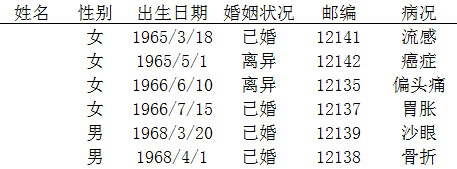
\includegraphics[width=5in]{chap1/anonymity1}
	\bicaption[fig:anonymity1]{图}{隐藏关键属性后的个人信息表}{Fig.}{Personal information form after hiding the key attributes}
\end{figure}

\begin{figure}[!htp]
	\centering
	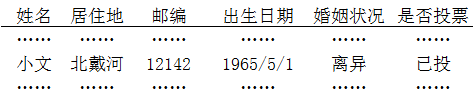
\includegraphics[width=5in]{chap1/anonymity3}
	\bicaption[fig:anonymity3]{图}{投票登记表}{Fig.}{Voting registration form}
\end{figure}


匿名化是隐私保护算法的主要实现技术之一,主要通过“抑制”和“泛化”操作分别达到隐藏关键属性和抽象敏感属性的保护手段,如删除显示标识符就属于抑制操作。最具代表性的匿名化算法是L.Sweeney和P.Samarati提出的$k$-匿名($k$-anonymity)\cite{k-anonymity}。它定义准标识符(Quasi-Identifies,QI)来表示那些能够与外表进行链接以标识个体身份的属性或属性组合,如图\ref{fig:anonymity1}的属性组{性别,出生日期,婚姻状况,邮编}就是个人信息表的QI。显然,QI的定义是依赖于外表信息的,对于同一个隐私表可能由于不同的外表的存在定义了不同的QI。$k$-匿名算法旨在通过匿名处理后的隐私表的每条记录至少与其他$k$-1条记录具有完全相同的QI属性值,这样在链接攻击时攻击者得到的元组中,在每个QI属性上至少包含了$k$条相同属性值的记录,因此无法唯一区分个体身份。

对图表\ref{fig:anonymity1}进行$k$=2的2-匿名处理后得到图表\ref{fig:anonymity2},邮编和出生日期基于数值型泛化技术予以抽象处理,用更大的取值范围代替原值。可以看到泛化处理在保护隐私的同时带来了信息的损失,如何减小匿名化算法的信息缺损(information loss)\cite{Bottom-up generalization}\cite{Top-down specialization}成了优化匿名保护算法的一个重要研究点。

\begin{figure}[!htp]
	\centering
	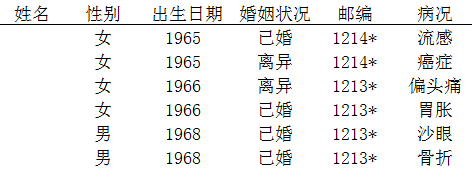
\includegraphics[width=5in]{chap1/anonymity2}
	\bicaption[fig:anonymity2]{图}{2-匿名化处理后的个人信息表}{Fig.}{personal information form with 2-anonymity}
\end{figure}

\subsection{面向分类应用的差分隐私算法}  %firedman

在分类需求的数据挖掘模型中,可以从训练数据中学习到有用的经验规则,但是在分析数据的同时极有可能泄露隐私,结合差分隐私技术给这一领域提供了新的解决思路。

分类模型的典型代表是决策树模型。SuLQ ID3\cite{SuLQ}是基于ID3算法的交互式差分隐私模型,在选择分类属性时通过往熵值添加满足差分隐私的拉普拉斯噪音达到隐私保护的目的,并且它事先规定了决策树的树高,隐私预算按树高被均分到每层参与计算。就1.2.3节的例1.1背景,对于有m个类属性C的训练集S,在属性A(有k个属性值)上对其进行划分得到\{S$_{1}$,S$_{2}$,...,S$_{k}$\},在计算信息增益时需要计算S的熵值和由A划分后的熵值。SuLQ ID3在每次迭代选择属性的过程中,对类个数|C$_{i}$|(i=1,2,...,m)、划分后的子集大小|S$_{j}$|(j=1,2,...,k)等计数值上添加拉普拉斯噪音,分别得到|$\widetilde{C_{i}}$|,|$\widetilde{S_{j}}$|等加噪结果。下式描述了SuLQ ID3中信息增益的计算,上方带波浪号表示添加了拉普拉斯噪音处理后的结果:
\[
\begin{split}
	En\widetilde{tro}py(S) &= -\sum_{i=1}^{m}\frac{|\widetilde{C_{i}}|}{|\widetilde{S}|}\log_{2}(\frac{|\widetilde{C_{i}}|}{|\widetilde{S}|})\\
	En\widetilde{tro}py_{A}(S) &= \sum_{i=1}^{k}\frac{|\widetilde{S_{i}}|}{|\widetilde{S}|}En\widetilde{tro}py(S_{i})\\
	Gain(S,A) &= En\widetilde{tro}py(S)-En\widetilde{tro}py_{A}(S)
\end{split}	
\]
显然,SuLQ ID3存在着不足:(1)这种往每个计数值直接加噪音的方式粒度太细,累加的噪音使得属性的选择变得不那么准确,同时也影响了下层的属性选择结果,那么在决策树逐层构建的过程中产生的放大效果严重影响了模型的分类准确度。(2)当数据集属性较多即树高定义较大时,不得不把隐私预算切分的比较细,由于噪音量大小与每层的隐私预算成反比,又进一步影响了属性选择的准确度。

针对SuLQ ID3的缺点,同为交互式差分隐私框架的DiffP-C4.5\cite{diffp-c4.5}在C4.5算法的基础上利用指数机制对此进行了优化。DiffP-C4.5算法先计算每个待选择属性的信息增益(不加噪音),把信息增益值作为指数机制的打分函数并与隐私预算、隐私敏感度一起参与计算,最后输出此属性的打分值,并以此打分值作为此属性被选中的概率。过程如图\ref{fig:diffp-c45}。

\begin{figure}[!htp]
	\centering
	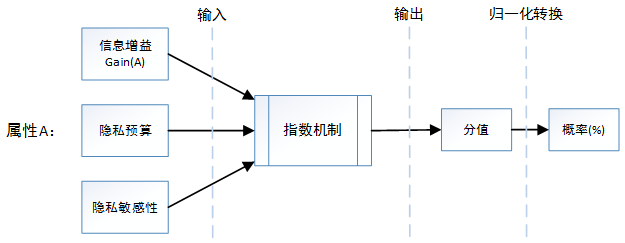
\includegraphics[width=5in]{chap1/diffp-c45}
	\bicaption[fig:diffp-c4.5]{图}{Diffp-C4.5选择属性的核心计算过程}{Fig.}{The core computational procedure of Diffp-C4.5 in selecting attribute}
\end{figure}

不同于SuLQ ID3和DiffP-C4.5,DiffGen\cite{DiffGen}采用了非交互式框架,并基于指数机制构建分类模型,最后发布匿名化数据集。此算法作为本文优化算法的基础,将在后边章节详细介绍。

\subsection{维度灾难}

数据纬度(dimension)问题一直是数据处理及应用算法中的难点问题,在面向数据挖掘应用的差分隐私算法中同样如此。为了便于数据统计,列联表(contingency table)、边界表(margin)和立方表(Cuboid)是常见的统计方式,但是数据维度会随着数据集属性的数量及每个属性的属性值个数的增加而变大,引起时间和空间复杂度问题。

\begin{figure}[!htp]
	\centering
	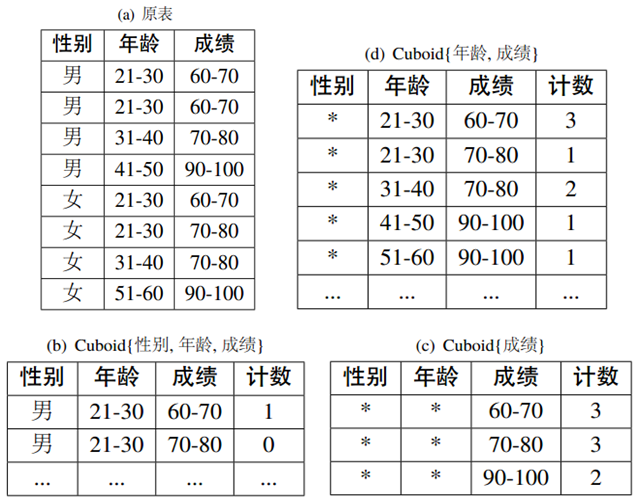
\includegraphics[width=5in]{chap1/cuboid}
	\bicaption[fig:cuboid]{图}{立方表示例}{Fig.}{Sample Cuboid}
\end{figure}

%# -*- coding: utf-8-unix -*-
%%==================================================
%% chapter02.tex for SJTU Master Thesis
%% Encoding: UTF-8
%%==================================================

%1,展开差分隐私定义,laplace,讨论维度问题
%2,展开面向决策树的差分隐私设计,典型方案


\chapter{相关背景技术}
\label{chap:background}

\section{引言}

上一章描述了课题所涉及的背景知识及相关问题的研究现状,本章将介绍差分隐私理论知识及焦点问题。主要内容为差分隐私相关的数学定义和重要概念介绍与频率矩阵加噪模型描述。

\section{差分隐私}

\subsection{差分隐私定义}

%给定数据集$D$,另一数据集$D'$和它至多相差一条记录。
在差分隐私中,我们希望某个在数据集上的运算结果不因任意一条记录的改变而变化明显。也就是说,某个算法在改变前后的两个数据集上做运算,其输出上的差别不至于披露任意一条特定数据项。

\begin{defn}
	
($\varepsilon$\textsc{-差分隐私})\cite{Dwork Calibrating} 数据集$D$和$D'$至多相差一条记录,即$|D$$\triangle$$D'|$ $\leqslant$ 1。一个随机算法$\partial$满足$\varepsilon$-差分隐私,当且仅当对于$\partial$任意可能的输出$O$,我们有下式成立:

\begin{equation}
  \label{eq:res1}
	 Pr[\partial(D) = O] \leqslant e^{\varepsilon} \cdot Pr[\partial(D') = O]
\end{equation}


其中,$Pr$表示事件发生的概率,在此也表示隐私被披露的风险。$\varepsilon$为隐私预算,$\varepsilon$越小,算法的隐私保护程度越高。

\end{defn}

实现差分隐私的主要方法是对真实值添加噪音扰动,而噪音量的量级大小是由全局敏感性(Sensitivity)来定义。它表示数据集发生改变时,某一函数运算在输出结果上产生的最大距离。

\begin{defn}
	(\textsc{全局敏感性}\cite{Dwork Calibrating}) 数据集$D$和$D'$至多相差一条记录,即$|D$$\triangle$$D'|$ $\leqslant$ 1。函数$\mathcal{F}$的查询维度为d,并且有$\mathcal{F}$:$D \rightarrow \mathrm{R}^d$。那么,函数$\mathcal{F}$的全局敏感性$S(\mathcal{F})$定义为:
\begin{equation}
\label{eq:res2}
	S(\mathcal{F}) = \max \limits_{D,D'} \| \mathcal{F}(D) - \mathcal{F}(D') \|_{1}
\end{equation}

其中,$\|\cdot\|$表示$L_{1}$范数。
\end{defn}

\subsection{差分隐私实现机制}

基于全局敏感性,本课题涉及两种加噪算法:拉普拉斯机制(Laplace mechanism)和指数机制(Exponential mechanism)。

\begin{thm}
	\label{thm:res1}
	(\textsc{拉普拉斯机制}\cite{Dwork Calibrating}) 在数据集$D$中,有函数$\mathcal{F}$: $D\rightarrow \mathrm{R}^d$,若算法$\mathcal{M}$满足下式,则$\mathcal{M}$满足$\varepsilon$-差分隐私:
	\begin{equation}
	\mathcal{M}(D) = \mathcal{F}(D) + (\textit{Laplace}(S(\mathcal{F})/ \varepsilon)^d
	\end{equation}
	其中,\textit{Laplace}为标准的拉普拉斯分布,$S(\mathcal{F})/\varepsilon$决定噪音量级。
\end{thm}
例如,当$\mathcal{F}$为求和函数时,S($\mathcal{F}$)=1,此时$\mathcal{M}(D) = \mathcal{F}(D) + (\textit{Laplace}(1/\varepsilon)^d$。

指数机制通过设计打分函数对属性进行打分计算,分值越高就有越大的概率被选中。
\begin{thm}
	\label{thm:res2}
	(\textsc{指数机制}\cite{exponential}) 有数据集$D$,打分函数$\mathcal{F}$: ($D$ $\times$ $O$)$\rightarrow$ $\mathrm{R}$,对每个输出项o$\in$ $O$都对应一个打分值。对于若算法$\mathcal{M}$满足下式,则$\mathcal{M}$满足$\varepsilon$-差分隐私:
	\begin{equation}
	\mathcal{M}(D,\mathcal{F}) = \{o \in O: Pr(o)\wasypropto exp(\frac{\varepsilon\mathcal{F}(D,o)}{2S(\mathcal{F})}) \}
	\end{equation}
	其中,S($\mathcal{F}$)为打分函数$\mathcal{F}$的全局敏感性,Pr(o)表示返回输出项o的概率。
\end{thm}
在决策树分类算法中,常用的打分有信息增益,基尼指数等。通过算法$\mathcal{M}$得到候选属性的概率值分布,之后按照概率抽取属性。

\subsection{差分隐私性质与误差方差}

对于不同组合关系的数据集,差分隐私具有序列(垂直)组合性质和并行(水平)组合性质。

\begin{lem}
	序列组合性质(Sequential composition)\cite{composition}随机算法$A_{i}$满足$\varepsilon_{i}$-差分隐私,则一系列算法$A_{i}$在数据集$D$上的序列组合满足$\sum\limits_i \varepsilon_{i}$-差分隐私。
\end{lem}

\begin{lem}
	\label{parallel}
	并行组合性质(Parallel composition)\cite{composition}随机算法$A$满足$\varepsilon$-差分隐私,数据集$D$被划分为一系列不相交的子集$D_{i}$,则算法$A$在每个数据集$D_{i}$上的操作$A(D_{i})$均满足$\varepsilon$-差分隐私。
\end{lem}


噪音的扰动虽然满足了差分隐私定义,但降低了数据集的准确性,需要一种衡量准确性损失的度量公式。误差方差是常用的度量公式,用来衡量原数据集分布和加噪数据集分布间的偏差,定义如下。
\begin{defn}
	\label{thm:error}
	(\textsc{误差方差}$error_{var}$\cite{Dwork Calibrating}) 在数据集$D$中,有查询函数$\mathcal{F}$: $D\rightarrow \mathrm{R}^d$且满足拉普拉斯机制,$\mathbb{E}$为方差,则查询的第i个元素的误差方差$error_{var}^{i}$及对整个查询Q的误差方差为
	\begin{eqnarray}
	&error_{var}^{i} = \mathbb{E}(\textit{Laplace}(S(\mathcal{F})/ \varepsilon)^2) = 2\frac{S(\mathcal{F})^2}{\varepsilon^2}\\
	&error_{var}^{Q} = \sum\nolimits_{i \in Q}error_{var}^{i}
	\end{eqnarray}
	其中,\textit{Laplace}为标准的拉普拉斯分布,$S(\mathcal{F})$为全局敏感性。
\end{defn}

例如,当$\mathcal{F}$为计数函数时全局敏感性为1,对于n个元素的查询Q,$error_{var}^{Q}$ = n$\mathbb{E}(\textit{Laplace}(S(1)/ \varepsilon)^2)$ = 2n/$\varepsilon^2$。

\section{频率矩阵及问题表述}

频率矩阵是数据处理领域中一种基本的统计模型,基于频率矩阵实现的差分隐私算法满足了基本的隐私保护需求,但在分类应用中,范围计数查询需求引发了新问题——基于单位行项的应答查询模式引起的噪音线性叠加问题。%随着查询维度的增加,累加的噪音值不断逼近真实值,严重影响数据使用性能的扩展性---这也是本课题的焦点问题。
本节先介绍频率矩阵模型,接着对数据维度、查询维度进行量化表述,并分析频率矩阵的应答查询模式。

\subsection{频率矩阵}

继续以例\ref{exmp_cuboid}为示例,原表的频率矩阵为取全属性的立方表,即Cuboid{性别,年龄,成绩}。如图\ref{fig:frequency}(a)为原表,\ref{fig:frequency}(b)为其对应的频率矩阵。可以看到,频率矩阵是枚举原表中所有属性(包括类属性)的组合情况,并统计相关的计数情况,通常情况下频率矩阵是大于原表的。

\begin{figure}[!htp]
	\centering
	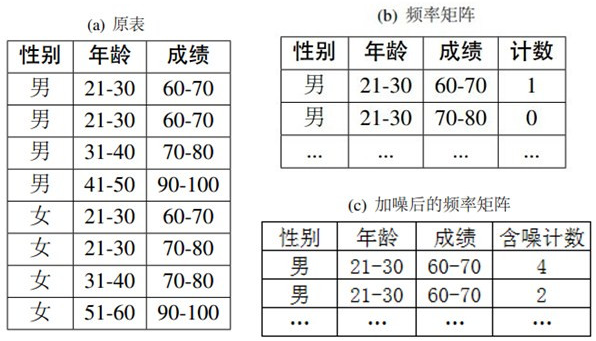
\includegraphics[width=5in]{chap2/frequency}
	\bicaption[fig:frequency]{图}{频率矩阵示例}{Fig.}{Sample frequency matrix}
\end{figure}

频率矩阵对原表条目进行了组织,便于数据的管理和查询。因此,本文的“数据集”通指组织成频率矩阵形式的数据集,而不是原表。频率矩阵中的每一行称之为“行项”(Entry),如表\ref{fig:frequency}(b)的\{“男”,21-30,60-70,1\}为一个行项。

\subsection{频率矩阵加噪模型}

本章节将对\ref{sec:weidu}节的查询维度问题进行量化表述,并说明基于频率矩阵的差分隐私算法的应答查询模式。

\subsubsection{数据维度}
数据维度在差分隐私算法研究中一般用数据域尺寸(Domain size)来表示。数据集D有n个非空行项,n$\in$ Z$^{+}$,并且有d个属性\{A$_{1}$,A$_{2}$,...,A$_{d}$\},每个属性A$_{i}$(i=1,2,...,d)有|A$_{i}$|个属性值。D的数据域尺寸表示为M,则M = \(\prod\limits_{i = 1}^d {|A{_i} |}\)且M $\gg$ n。

\subsubsection{查询维度}
查询维度是衡量查询项所涉及的属性数目。一查询请求Q(A$_{k}$, A$_{k+1}$, ..., A$_{j}$),其中j,k$\in$ Z$^{+}$,j $\geqslant$ k且j $\geqslant$ d,则Q的查询维度为$j-k$。

\subsubsection{应答查询模式}
\label{chap2_Linaer}
应答查询模式在本课题研究中指的是,为响应范围计数查询需求所采用的查表、累加等操作并最终返回应答结果的方式。频率矩阵的应答查询模式为查找符合查询范围的相关行项并对每个行项的计数值做累加运算,最后返回运算结果。以下定义这种应答查询模式为线性累加的应答查询模式$LinearR$。

\begin{defn}
	(\textsc{线性累加的应答查询模式$LinearR$}) 有d维类属性分布的数据集$D$,范围查询$R_{query}$,对于其中某数据项$D_{i}$,查询函数$\mathcal{F}$:$D_{i} \rightarrow \mathrm{R}^d$,应答返回集合$Answer$,线性累加的应答查询模式$LinearR$定义为:
	\begin{equation*}
	\label{eq:linear_response}
		\begin{split}
			\text{当}\forall D_{i},D_{j} \in Answer, i \neq j, \text{则} D_{i} &\cap D_{j} = \varnothing,\text{且 }
			R_{query} = \bigcup\limits_{\forall D_{i} \in Answer} D_{i}\\
			\text{那么,有}LinearR &= \sum\limits_{\forall D_{i} \in Answer} \mathcal{F}(D_{i})
		\end{split}
	\end{equation*}
\end{defn}

在$LinearR$中,由于单个行项之间是互不相交的(在每个属性上具有不同的属性值分布),因此这种应答结果是以行项为单位的累加计算之和。

\subsubsection{频率矩阵加噪模型}

某查询请求是对\{A$_{k}$, A$_{k+1}$, ..., A$_{j}$\}以外的某一属性值的查询,那么根据频率矩阵特性,在D中查表涉及到的行项数至少为E = \(\prod\nolimits_{i \in (1,d) - (k,j)} {|A{_i} |} \)。例如,查询表\ref{fig:frequency}(b)中男性的计数量,此时Q = \{年龄,成绩\},E = 4x3,显然需要遍历“性别”属性以外的所有属性组合,最终的结果需要对E个数值进行|E-1|次累加操作。

可以看到,M决定了Q的查询维度范围,并且随着查询维度的增加,近乎指数级增长的行项数量级会使得数据集D的查表过程变得复杂,时间复杂度为O(E)。在差分隐私算法中,由于拉普拉斯噪音的引入,还带来了噪音叠加问题。

在典型的基于频率矩阵的差分隐私算法中\cite{Dwork Calibrating},Dwork等人通过在频率矩阵的每个行项计数值上添加拉普拉斯噪音的方法实现差分隐私保护,如图\ref{fig:frequency}(c)。在应答范围查询时,根据其基于行项的应答查询模式,此方案的全局敏感性为1,因此对于单位行项查询结果的噪音方差为$\Theta$(1)。那么在涉及E个行项的范围查询Q中,应答结果的总噪音方差为多少呢?

若原计数值为C,加噪之后的噪声值$\tilde{C}$为
\[
\tilde{C} = C + Laplace(1/\varepsilon)^d
\]
在Q的查询结果中,对比加噪前后引入的噪音总量:原计数总量$\sum{C}$ = \(\prod\nolimits_{i \in (1,d) - (k,j)} {C{_i}} \),加噪之后的计数总量$\sum{\tilde{C}}$ = \(\prod\nolimits_{i \in (1,d) - (k,j)} {C{_i}} \) + E$\cdotp$Laplace(1/$\varepsilon$)$^d$。那么,引入的噪音干扰为
\[
|\sum{\tilde{C}} - \sum{C}| = E \cdotp Laplace(1/\varepsilon)^d
\]
因此,应答结果的总噪音误差方差为$\Theta$(E)。

可以看到,以行项为单位的独立加噪和线性累加的应答查询模式$LinearR$,决定了以线性累加运算来得到终值的解决办法。在求真实值的|E-1|次运算中,噪音也发生了同规模运算,并且与所涉及的行项数呈线性相关。噪音的误差方差与范围计数查询的查询维度成正比,因此,随着查询维度的增加,返回结果的可用性将大大降低。

\section{本章小结}

本章节细致介绍了频率矩阵模型,并且量化表述了查询维度引起的噪音叠加问题。本论文中的“频率矩阵加噪模型”指的就是Dwork等人采用的传统差分隐私加噪模型——往频率矩阵的每个行项计数加拉普拉斯噪音的方式。在后文还将进一步分析此模型,说明它的一维直方图特性。

本文接下来的章节将介绍解决思路及方法实现——对于非单位长度的查询请求,揭示经典的非交互式差分隐私算法中存在着和频率矩阵加噪模型一致的噪音线性叠加问题。所涉及的行项集是无法减免的,但是可以通过匿名数据属性间的一致性关系,调整噪音的分布,改变线性累加的应答查询模式($LinearR$),从而尽可能减少噪音的线性叠加现象,提升发布数据的可用性。



%# -*- coding: utf-8-unix -*-

\raggedbottom
\chapter{基础算法与优化思路}
\label{chap:algorithm}

\section{引言}
经典的非交互式差分隐私匿名算法DiffGen是本课题优化算法设计的基础。本章节有针对性地对DiffGen算法进行介绍分析,并揭示其缺陷模型本质为频率矩阵加噪模型。接下来探讨针对一维直方图发布方式的基于一致性约束的优化方案$BoostH$,总结其应用特性,并分析与DiffGen的联系和启发思路。
这也给频率矩阵模型问题提供了解决方案,并结合DiffGen算法,为接下来的优化算法做铺垫。

\section{基础算法概览}

DiffGen算法是由Mohammed等人于2011年提出的一个非交互式差分隐私匿名算法\cite{DiffGen},基于分类树结构和指数机制构建重匿名数据集,其性能优于SuLQ-basedID3和DiffP-C4.5,但仍存在着不足。
%本节的示例均基于例\ref{chap3_exmp}的背景,表述如下:
\begin{exmp}
	\label{chap3_exmp}
	某公司有8位应聘者,对“国籍”、“年龄”以及是否被录用统计如表\ref{chap3_table}(a),类属性为“是否被录用”。
\end{exmp}

\begin{table}[!hpb]
	\label{chap3_table}
	\centering
		\bicaption[tab:firstone]{表}{应聘者统计表}{Table}{The statistical table for candidates}
	\subtable[统计表]{
		\begin{tabular}{|c|c|c|}
			\hline
			$\textbf{国籍}$ & $\textbf{年龄}$ & $\textbf{是否被录用}$ \\
			\hline
			中国 & 18 & 否 \\
			\hline
			蒙古 & 21 & 是 \\
			\hline
			伊朗 & 27 & 否 \\
			\hline
			以色列 & 35 & 否 \\
			\hline
			以色列 & 29 & 是 \\
			\hline
			中国 & 39 & 是 \\
			\hline
			蒙古 & 22 & 否 \\
			\hline
			中国 & 28 & 否 \\
			\hline
		\end{tabular}}
		\qquad
		\subtable[泛化处理后的统计表]{%
			\begin{tabular}{|c|c|c|}
				\hline
				$\textbf{国籍}$ & $\textbf{年龄}$ & $\textbf{类属性计数(录用分布)}$ \\
				\hline
				东亚 & [15-25) & 3 (1是2否) \\
				\hline
				东亚 & [25-40) & 2 (1是1否) \\
				\hline
				西亚 & [15-25) & 0 (0是0否) \\
				\hline
				西亚 & [25-40) & 3 (1是2否) \\
				\hline
			\end{tabular}}
		\end{table}

\subsection{泛化技术与匿名树}

泛化技术是匿名算法实现的关键技术,在DiffGen中通过匿名树(Taxonomy tree)来组织每个属性下属性值的匿名层级关系,如图\ref{fig:taxonomy}所示。原属性作为叶节点,通过指定更一般的泛化域(Dom),自底向上地构建匿名树,如中国与蒙古的泛化域为东亚。
对于离散属性(Categorical attribute)如“国籍”,采用抽取共性的方式进行逐层泛化;对于连续属性(Numerical attribute)如“年龄”,通过更大的连续区间进行泛化。表\ref{chap3_table}(b)是泛化处理后的统计结果。
从根节点自顶向下来看,匿名树定义了一套划分规则(Partition guidelines),指导每个泛化属性如何分裂,如“东亚”的分裂趋势为分成“中国”和“蒙古”。从叶节点自底向上来看,匿名树定义了一套抽象规则(Generation guidelines),显示了父子节点间的包含关系。
%显然匿名树中的属性值是不重复。

匿名规则需要数据发布者自己定义,算法读取语义文件并构建匿名树作为属性分裂时的划分依据。匿名树最底层的非叶子节点用气泡框标识,表示最“细”的发布属性值,最多发布到此为止。

\begin{figure}[!htp]
	\centering
	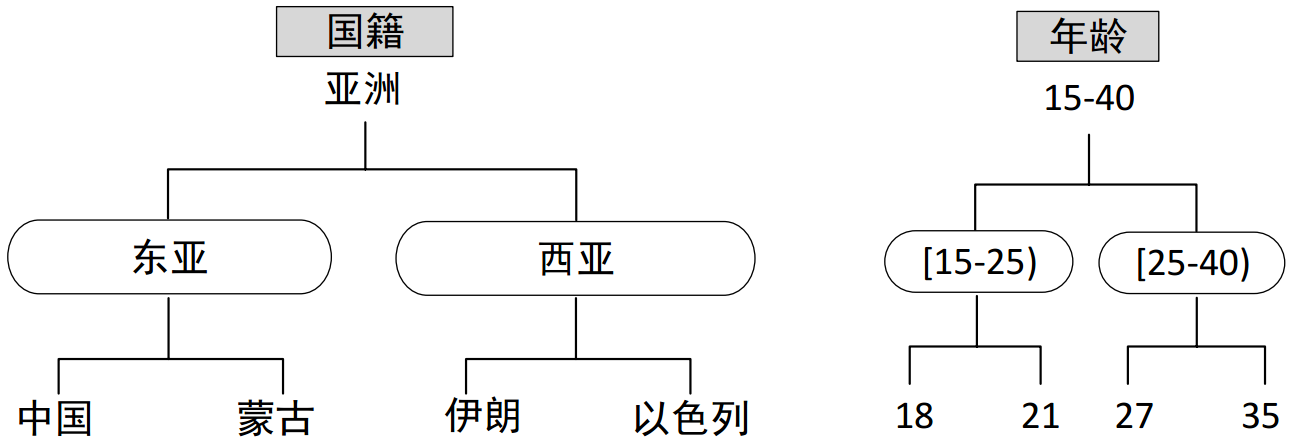
\includegraphics[width=5in]{chap3/taxonomy}
	\bicaption[fig:taxonomy]{图}{属性“国籍”和“年龄”的匿名树}{Fig.}{The taxonomy tree for 'Country' and 'Age'}
\end{figure}


\subsection{算法概述}

面向分类应用的非交互式差分隐私匿名算法DiffGen主要的流程为:(1)为每个属性定义匿名树语义文件,并定义树高。(2)基于决策树算法构建“DiffGen分类树”并逐层划分数据集。(3)由叶节点的类属性计数生成发布数据集。
整个流程伪代码\ref{total_diffgen}概括如下:

\begin{algorithm}[H]
	\caption{DiffGen算法流程} 
	\label{total_diffgen}
	\begin{algorithmic}[1]
		\REQUIRE 隐私代价$\varepsilon$,树高$Hight$,数据集,匿名树集合。
		\ENSURE 发布数据集。
		\STATE 定义合理数据结构处理数据集和匿名树森林,并建立相应联系
		\STATE 初始化分类树根节点,记当前树高为$h$
		\WHILE{$h++$ < $Hight$} 
		\STATE 基于决策树算法,逐层选择属性、分裂当前节点并划分父节点数据集,构建分类树。
		\ENDWHILE
		\STATE 在分类树叶子节点的类属性计数上添加拉普拉斯噪音,全局敏感性为1。
		\STATE 遍历叶节点,根据类属性计数值生成匿名化数据集
		\RETURN 发布数据集
	\end{algorithmic}
\end{algorithm}

其中,DiffGen分类树是数据集划分、属性选择的基础结构。

\subsection{算法框架}

在这个阶段,DiffGen算法依据匿名树的分裂规则,采用决策树算法通过指数机制逐层选择分裂属性,并作数据集划分,构建完整的分类树,最后在叶节点加噪并发布数据集。为了更清楚地展示这个过程以及理解DiffGen算法伪代码,继续使用前文公司应聘的例子做说明。

DiffGen算法以匿名树作为属性划分规则,采用决策树算法通过指数机制逐层选择分裂属性,并作数据集划分,构建完整的DiffGen分类树,最后在叶节点加噪并发布数据集。图\ref{fig:diffgen}展示了例\ref{chap3_exmp}背景下的算法工作过程。算法\ref{diffgen}对DiffGen算法进行了完整描述,其中$Cut_{i}$表示在当分类树树高为i时,所有匿名树中可分裂的属性集合。如仅有根节点时,$Cut_{1}$=\{亚洲,[15-40)\};而选取分裂属性亚洲后,$Cut_{2}$=\{东亚,西亚,[15-40)\}。$u(D,\cdotp)$表示打分函数,$S(u)$为其全局敏感性。

\begin{algorithm}
	\caption{DiffGen算法} 
	\label{diffgen}
	\begin{algorithmic}[1]
		\REQUIRE 隐私代价$\varepsilon$,树高$Height$,数据集$D$。
		\ENSURE 新的匿名数据集$\hat{D}$。
		\STATE 初始化分类树根节点和$Cut_{i}$集合,此时i=1
		\STATE 按树高切割$\varepsilon$,统计连续属性个数为$A_{Pr}^{n}$,$\varepsilon$' $\leftarrow$ $\frac{\varepsilon}{2(|A_{Pr}^{n}|+2Hight)}$
		\STATE 对$Cut_{i}$里的每个连续属性$v_{n}$,计算其分裂点$p$,分裂点$p$的选中概率 $\wasypropto$ exp($\frac{\varepsilon\textasciiacute}{2S(u)}$$u(D,v_{n})$)
		\STATE 对所有的属性$v$, $\forall$$v$ $\in$ $Cut_{i}$,计算分值
		\FOR{i = 1 to $Hight$}
		\STATE 按分值选择属性$v$,$v$$\in$ $Cut_{i}$,且$v$的选中概率$\wasypropto$ exp($\frac{\varepsilon\textasciiacute}{2S(u)}$$u(D,v)$)
		\STATE 根据$v$的匿名树分裂节点$v$,$v$$\rightarrow$$child(v)$
		\STATE $Cut_{i}$ $\leftarrow$ $Cut_{i}$$ - $$v$,$Cut_{i}$ $\leftarrow$ $Cut_{i}$ $\cup$ $child(v)$
		\STATE 对$Cut_{i}$里的新出现的连续属性$v_{n}$,计算其分裂点$p$,分裂点$p$的选中概率 $\wasypropto$ exp($\frac{\varepsilon\textasciiacute}{2S(u)}$$u(D,v_{n})$)
		\STATE 对所有的属性$v$, $\forall$$v$ $\in$ $Cut_{i}$,更新分值
		\ENDFOR
		\RETURN 在叶子节点的数据项上,每个类属性计数为$C$,返回($C$+$\textit{Laplace}$(1/$\varepsilon$))
	\end{algorithmic}
\end{algorithm}


\begin{figure}[!htp]
	\centering
	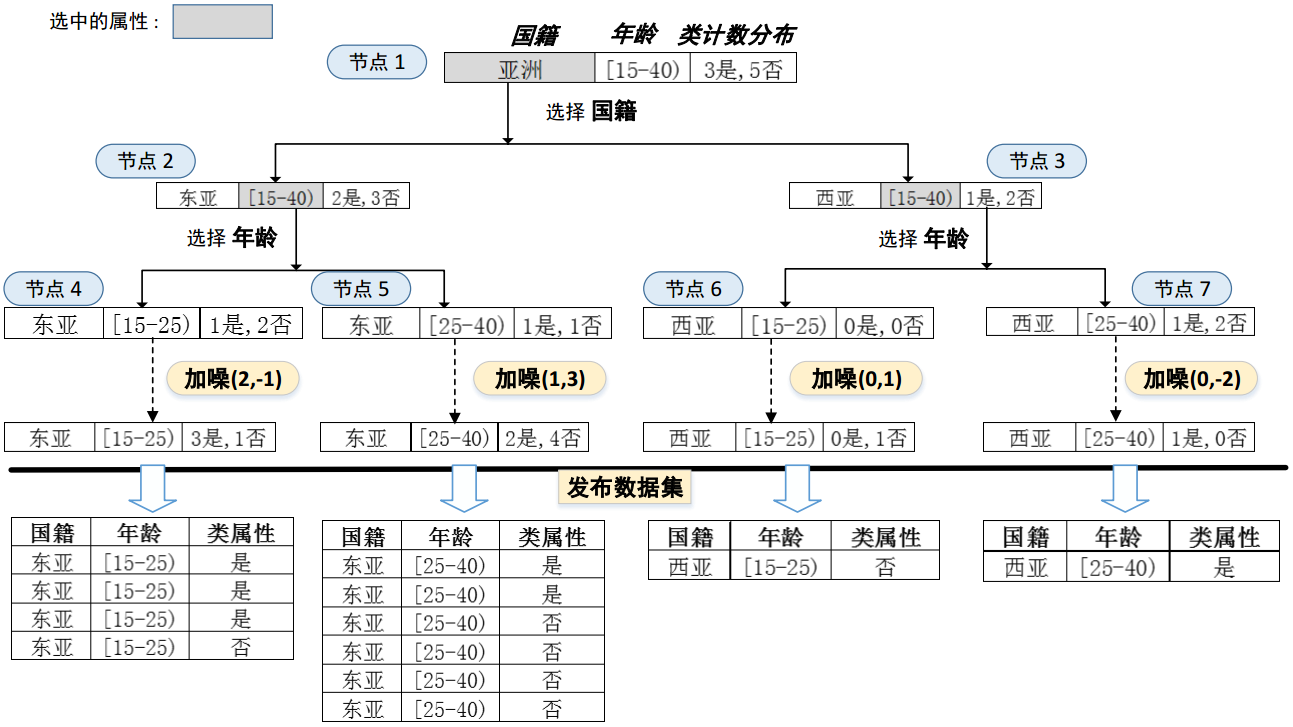
\includegraphics[width=6.2in]{chap3/diffgen}
	\bicaption[fig:diffgen]{图}{基于DiffGen算法的数据集发布流程概述}{Fig.}{The release process for dataset based DiffGen}
\end{figure}

结合算法\ref{diffgen}与图\ref{fig:diffgen},DiffGen的运行过程概括如下:

\begin{enumerate}
	\label{process}
	\item 事先定义DiffGen分类树的树高$Height$。在第1行做初始化,组合所有匿名树的根节点属性值作为分类树的根节点与$Cut_{i}$的初始值。选取分裂属性和处理连续属性分裂点时需要消耗隐私预算,因此在第2行对隐私预算进行了切分。
	\item 数据集归属节点的选择方法为:每个数据项根据属性值包含关系,归入相应的节点。例如,由各匿名树根节点属性值构成了“节点1”。对于数据项\{中国,18,否\},根据各匿名树结构有“中国”$\in$“亚洲”,“18”$\in$“[15-40]”,因此它归入“节点1”。在DiffGen分类树做节点分裂时,被分裂节点上的数据项按此方法归入下层对应的节点。
	\item 在5-10行的每次迭代中,需要先对待选择属性集$Cut_{i}$的每个属性计算分值并对连续属性处理进行处理,然后通过指数机制按概率挑选属性;在第8,9,10行为下一次属性选择做更新操作。分裂节点的同时伴随着第2步的方法进行数据集的划分。例如,节点1选出属性“国籍”,根据匿名树划分为“东亚”和“西亚”,生成节点2和节点3,同时节点1上的数据集也归入相应的节点。
	\item 对节点来说,有两种情况不发生节点分裂:(a)到迭代上限,即树高$Height$。(b)选中属性在此节点的属性值是匿名树的最“细”划分限度——“气泡框”。
	\item 以图\ref{fig:diffgen}以中间的粗直线为界,上半部分为完整的DiffGen分类树,下半部分为数据发布过程。算法的第12行在每个叶节点类属性计数上添加独立的拉普拉斯噪音,并返回。最后发布统计情况,发布的新数据集如表\ref{chap3_table2}的(a)(b)(c)(d)所示。
\end{enumerate}

\begin{table}[!hpb]
	\label{chap3_table2}
	\centering
	\bicaption[tab:firstone]{表}{DiffGen算法处理后的发布数据集}{Table}{The realesed dataset after DiffGen}
	\subtable[数据项1]{
		\begin{tabular}{|c|c|c|}
			\hline
			$\textbf{国籍}$ & $\textbf{年龄}$ & $\textbf{是否被录用}$ \\
			\hline
			东亚 & [15-25) & 是 \\
			\hline
			东亚 & [15-25) & 是 \\
			\hline
			东亚 & [15-25) & 是 \\
			\hline
			东亚 & [15-25) & 否 \\
			\hline
		\end{tabular}}
		\qquad
		\subtable[数据项2]{%
		\begin{tabular}{|c|c|c|}
			\hline
			$\textbf{国籍}$ & $\textbf{年龄}$ & $\textbf{是否被录用}$ \\
			\hline
			东亚 & [25-40) & 是 \\
			\hline
			东亚 & [25-40) & 是 \\
			\hline
			东亚 & [25-40) & 否 \\
			\hline
			东亚 & [25-40) & 否 \\
			\hline
			东亚 & [25-40) & 否 \\
			\hline
			东亚 & [25-40) & 否 \\
			\hline
		\end{tabular}}
		\qquad
		\subtable[数据项3]{%
		\begin{tabular}{|c|c|c|}
			\hline
			$\textbf{国籍}$ & $\textbf{年龄}$ & $\textbf{是否被录用}$ \\
			\hline
			西亚 & [15-25) & 否 \\
			\hline
		\end{tabular}}
		\qquad
		\subtable[数据项4]{%
		\begin{tabular}{|c|c|c|}
			\hline
			$\textbf{国籍}$ & $\textbf{年龄}$ & $\textbf{是否被录用}$ \\
			\hline
			西亚 & [25-40) & 是 \\
			\hline
		\end{tabular}}
\end{table}


\subsection{算法缺陷}

根据分类树的构建方法,每个叶节点中的数据集拥有相同的属性值分布,因此组织所有叶节点数据时每个叶节点中的数据存放于同一行中。如图\ref{fig:diffgen}的下半部分所示,这其实就是一个二维类属性分布的频率矩阵。那么,DiffGen往叶节点的每个类分布加噪的方式其实就等同于频率矩阵加噪模型中往每个行项加噪的做法。

在查询应答模式上,DiffGen采用的是与频率矩阵加噪模型一样的线性累加的应答查询模式($LinearR$)。首先DiffGen的叶节点集满足差分隐私的水平组合性质\ref{parallel}(Mohammed等人的论文\cite{DiffGen}已证明),每行数据项,即每个叶节点间均两两不相交(证明在下个章节),因此叶节点上的加噪和应答是相互独立的,其拉普拉斯噪音的敏感性为一常量。其次,发布数据集的结构决定了基于行项的处理模式——直接发布加噪后的二维类属性分布的频率矩阵。
例如,在发布数据集上运行决策树分类算法产生范围计数查询需求,计算总熵值时需要对全属性分布的计数情况进行累加计算,此时含噪的[数据项\{1,2,3,4\}]发生线性叠加;当计算“东亚”的熵值时,需要[数据项\{1,2\}]的线性叠加运算。

因此,在范围查询需求的应用中,DiffGen模型的本质和前文所讨论的频率矩阵加噪模型是一致的,以行项级别粒度的加噪方式会严重制约发布数据的可用性。


\section{一致性特性}

Michael Hay等人提出了利用一致性约束提升直方图方式(universal histogram)发布数据可用性的方法\cite{boosting},为了书写方便本文称此优化方法为$BoostH$(boost histograms)。$BoostH$并未减少噪音量,而是通过对噪音分布的后置求精处理,使得对于任意范围的查询请求,应答结果均具有较高的准确度及可用性。在面向分类应用的范围计数查询需求方面,本小节分析了它与DiffGen算法的联系并总结启发思路。

\subsection{直方图发布方式}  %要说一下 DiffGen的频率矩阵加噪模型具有一维直方图特性!!!

在经典的LP\cite{Dwork Calibrating}方法中,直方图发布方式使用“分箱(Bin)”思想:先将属性值范围切割成若干个箱子,然后将数据集根据属性值放入不同的箱子构成一直方图,最后在每个柱状条(箱子)的计数上添加满足差分隐私的噪音,并发布数据。

在数据集$D$的直方图中,有$n$个柱状条,每个柱状条的属性值范围为$Bin_{i}$,其计数为$C(Bin_{i})$,加噪后计数为$\tilde{C}(Bin_{i})$,则一维直方图的数据发布格式$L_{unit}$与$\tilde{L}_{unit}$为
\[
\begin{split}
	L_{unit} = \{C(Bin_{1}),C(Bin_{2}),...,C(Bin_{n})\}\\
	\tilde{L}_{unit} = \{\tilde{C}(Bin_{1}),\tilde{C}(Bin_{2}),...,\tilde{C}(Bin_{n})\}	
\end{split}
\]
根据表\ref{chap3_table}(a)的“年龄”属性统计情况构建直方图\ref{fig:histogram},“人数”表示该年龄段参加应聘的总人数。将年龄值范围[15-40]以5为间距切割成5个“箱子”,每条数据根据年龄值归入相应的柱状条中。最后,在每个柱状条上添加拉普拉斯噪音并发布数据,其中$L_{unit} = \{C(Bin_{15-19}),C(Bin_{20-24}),C(Bin_{25-29}),C(Bin_{30-34}),C(Bin_{35-40})\}$ = $\{1,2,3,0,2\}$%由于柱状条的计数分布是相互独立的,因此噪音的全局敏感性为1。

\begin{figure}[!htp]
	\centering
	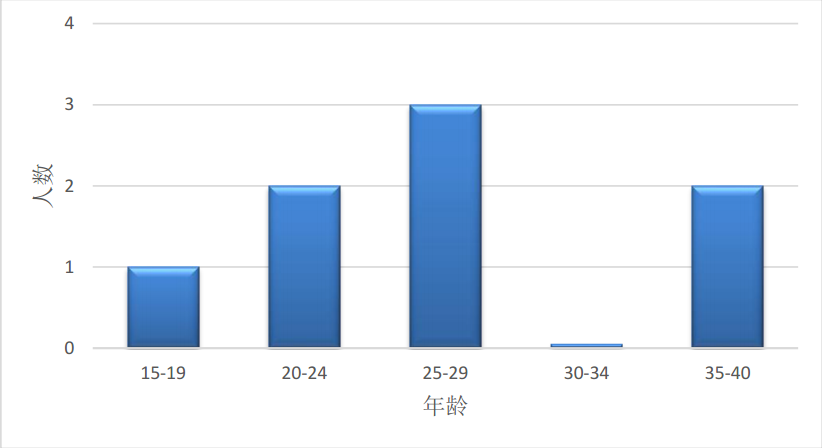
\includegraphics[width=5in]{chap3/histogram}
	\bicaption[fig:histogram]{图}{属性“年龄”的直方图显示}{Fig.}{The Histogram of attribute 'Age'}
\end{figure}

差分隐私中的直方图发布方式对于单位长度(Unit length)的查询能提供较好的支持,每个柱状条代表单位长度的计数情况,直接返回即可。但是对于范围查询请求来说,只能采用线性叠加的查询应答模式$LinearR$。由于每个柱状条的属性值区间是相互独立的,并且全局敏感性为一常量,因此直方图模型也遇到了频率矩阵加噪模型一样的问题。

\subsection{一致性特性}
\label{LP_publish}

就差分隐私直方图发布方式在范围查询中的噪音线性叠加问题,$BoostH$通过树状的辅助结构$BoostTree$,改变线性叠加的查询应答模式为树结构相关的搜索应答模式,并通过利用一致性约束对噪音分布进行优化。

图\ref{fig:histogram}的“年龄”直方图发布格式虽然是基于单位长度柱状条分布的$\tilde{L}_{unit}$,但是不同的年龄属性之间存在着一致性关系。图\ref{fig:consistency}呈现了这种关系,归纳了“年龄”的树状辅助结构$BoostTree$,利用了泛化技术处理属性值区间,把单位长度柱状条作为叶节点,自底向上构建树结构以完成对直方图的转换。图中的标号A,B,C,D,E对应原先直方图中的单位柱状条。此时由于属性值区间的包含关系,可从树结构中的父子节点对得到以下的一致性关系等式,${\it{C}}_{a-b}$表示属性值区间[$a-b$]的计数值:
\begin{equation}
\label{consistent_equal}
\begin{split}
&{\it{C}}_{15-24} = {\it{C}}_{15-19}+{\it{C}}_{20-24}\\
&{\it{C}}_{25-34} = {\it{C}}_{25-29}+{\it{C}}_{30-34}\\
&{\it{C}}_{15-34} = {\it{C}}_{15-24}+{\it{C}}_{25-34}\\
&{\it{C}}_{15-40} = {\it{C}}_{15-34}+{\it{C}}_{35-40}
\end{split}
\end{equation}

\begin{figure}[!htp]
	\centering
	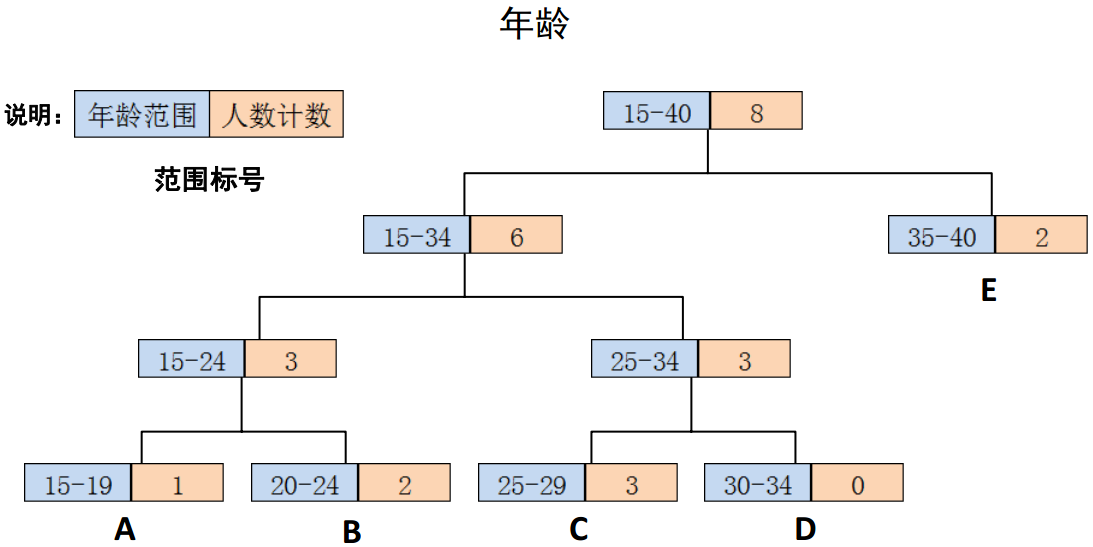
\includegraphics[width=5in]{chap3/consistency}
	\bicaption[fig:consistency]{图}{属性“年龄”的树状组织结构"BoostTree"}{Fig.}{The tree-organization structure 'BoostTree' for attribute 'Age'}
\end{figure}

%在直方图方式中,通过{$\widetilde{C}$} = {\it{C}} + Laplace(1/$\varepsilon$)给每个单位柱状条加噪音,并以累加操作响应非单位长度的范围查询。如查询年龄为[15-34],则返回结果({$\widetilde{C}_{A}$}+{$\widetilde{C}_{B}$}+{$\widetilde{C}_{C}$}+{$\widetilde{C}_{D}$})。但是
此时,对于年龄区间[15-34]的查询,通过等式\ref{consistent_equal}可以看到,若能直接返回{$\widetilde{C}_{15-34}$},从噪音叠加次数上来看,显然优于$\{\tilde{C}(Bin_{15-19})+\tilde{C}(Bin_{20-24})+\tilde{C}(Bin_{25-29})+\tilde{C}(Bin_{30-34})\}$。若由于噪音的不确定性,那至少可以提供min({$\tilde{C}_{15-34}$},{$\tilde{C}_{A}$}+{$\tilde{C}_{B}$}+{$\tilde{C}_{C}$}+{$\tilde{C}_{D}$})给用户。多种组合的选择无疑给发布数据带来了提升空间。

因此,自然的想法是改变基于叶节点的加噪方式为遍布$BoostTree$上所有节点的加噪,然后发布整个节点集供用户挑选更优的组合,即按某种节点遍历顺序发布具有一致性特性的树结构信息。假设树上有$ntree$个节点,这种发布格式$\tilde{L}_{all}$为
\begin{equation}
\label{L_allnodes}
\tilde{L}_{all} = \{\tilde{C}_{1},\tilde{C}_{2},...,\tilde{C}_{ntree}\}
\end{equation}
%因为一致性是属性值区间之间的内在属性,加噪操作改变的仅仅是数值。更具一般性,由于噪音数值的不确定性,我们可以选取min({$\widetilde{C}_{15-34}$},{$\widetilde{C}_{A}$}+{$\widetilde{C}_{B}$}+{$\widetilde{C}_{C}$}+{$\widetilde{C}_{D}$})作为应答返回,这无疑给发布数据提供了提升空间。

\subsection{BoostH的优化方案}
\label{BoostH}

但是,$\tilde{L}_{all}$的发布格式存在两个弊端:
\begin{itemize}
	\item[(1)] 给$BoostTree$的每个节点加噪之后,由于噪音的随机性使得节点间的一致性等式不再成立,例如绝大部分情况下{$\tilde{C}_{15-24}$}$ \neq ${$\tilde{C}_{15-19}$}+{$\tilde{C}_{20-24}$}。因此,用户无法从数值上分辨$\tilde{L}_{all}$中的一致性关系,这使得通过提供多个组合以提升结果精确度的方案失效。
	\item[(2)] 通过采用某种方案提供节点间的一致性关系,虽然能够提升发布数据准确度,但是这泄露了树结构、节点关系、内部节点等信息,发布数据集的安全性得不到保障。
\end{itemize}

因此$\tilde{L}_{all}$的发布格式不可行,但是其改变应答查询模式的思路是可取的。对于查询范围$R_{query}$,$BoostH$采用新的应答查询模式:寻找$BoostTree$中能够覆盖$R_{query}$的最小节点集合作为应答结果。例如,在图\ref{fig:consistency}中,当$R_{query}$ = \{[15-25]\},则返回节点集\{$\tilde{C}_{15-24}$,$\tilde{C}_{25-29}$\}。此方法能够有效避免噪音的线性叠加现象,但需要重新设计内部节点$\tilde{C}_{15-24}$的发布格式。

$BoostH$采用$\tilde{L}_{all}$的应答查询模式,重定义了全局敏感性,然后基于$BoostTree$结构对噪音分布进行后置处理,使得$BoostTree$上的含噪叶节点间重新满足\ref{consistent_equal}的一致性等式关系。重获一致性意味着任何内部节点可通过叶节点的线性累加获得,因此采用$\tilde{L}$的发布格式即可。

$BoostH$的这种方案解决了$\tilde{L}_{all}$的两大弊端。首先,重获一致性的$BoostTree$结构使得非叶结点的应答可通过叶节点数据项的叠加得到,这和直接返回非叶结点的效果是一样的。其次,未暴露内部节点信息,不影响安全性。此外,$BoostH$给新的应答查询模式定义了全局敏感性,并且噪音的调整仅仅是数值处理,因此的调整算法及数据发布过程并不违背差分隐私定义。这种基于一致性约束的噪音优化调整方案,能够用简单的直方图发布方式在范围查询需求中获得较好的准确性结果,且不是安全保障力度,其在应用背景、问题模型等方面与DiffGen有着密切的联系,启发了本课题DiffCon算法的设计思路。

%通过基于一致性约束的噪音优化调整过程,$BoostH$采用简单的直方图发布方式在响应范围查询请求的同时,达到了减免噪音叠加与确保数据结构安全性的目的。
%同样对于频率矩阵加噪问题,$BoostH$通过先树状辅助结构改变加噪方式,然后利用一致性特性调整噪音分布达到优化发布数据准确度的效果,并且未改变数据发布格式。



\subsection{框架适用性探讨}

根据上一节的论述,本小节对$BoostH$的基于一致性约束的优化方案与DiffGen算法的联系和启发进行总结:
\begin{enumerate}
	\item 模型基础。$BoostH$的直方图发布模型和DiffGen模型具有相同的模型特征——一维属性的计数统计特征。此模型特征的特点在于每个单位数据项仅代表一维属性范围,任意的范围查询能够通过数据项的叠加覆盖到,区别于多维属性直方图由于数据项表示范围的局限而无法完全覆盖的问题。
	虽然DiffGen的每个数据项包含多个属性,但是分类树的父子节点间存在完整的泛化包含关系,对于所有属性区间的查询均可通过叶节点的组合给予应答,因此本质上每个数据项的多维属性分布在组合应答关系中仍然体现出一维直方图特征。
	%各属性的范围查询均可以通过节点叠加完成,因此从X轴上看是多个一维属性直方图的组合。
	对于多维类属性分布,在Y轴上的行为可看是多个一维类属性直方图的组合。因此,DiffGen具有一维直方图特征。
	\item 问题背景。二者的性能瓶颈是相同的:均属于频率矩阵加噪模型问题。基于单位长度的加噪操作、采用$LinearR$的线性累加的应答查询模式,在面对范围计数查询需求时,存在着噪音等额叠加的核心问题。
	\item 优化思路。泛化技术和决策树分类方式决定了DiffGen分类树中存在一致性特性。匿名树的父子层级之间存在明确的泛化关系,使得一致性特性成了DiffGen分类树中父子节点间的固有属性。
	\item 差分隐私定义。应答查询模式的改变影响了全局敏感性,由于树状辅助结构的引入和一致性关系的存在,单位长度计数值之间再也不是相互独立的了——某一单位长度计数值的改变至少影响着它到根节点路径上的所有节点。
	\item 数据发布格式。由于重获一致性,$BoostH$未改变原先直方图的数据发布格式。对DiffGen来说,分类树的非叶子节点信息不仅揭露了分类树的属性选择和分类结构,更关键的是它揭示了算法中的匿名化技术细节。匿名化结构的暴露会从根本上破坏DiffGen算法,使其丧失隐私保护意义。因此,原先的仅发布单位数据项的做法应予以推崇。
	
\end{enumerate}

基于以上总结,在下一章节将详细介绍DiffCon算法的设计及实现。
%# -*- coding: utf-8-unix -*-
%%==================================================
%% conclusion.tex for SJTUThesis
%% Encoding: UTF-8
%%==================================================

\begin{summary}

这里是全文总结内容。

在前面的章节,我们已经介绍了面向分类应用的差分隐私算法在范围计数查询需求中存在的噪音线性叠加的问题,探讨了问题的频率矩阵加噪模型本质。接着详细介绍基础算法DiffGen与基于直方图发布方式的优化方案,DiffGen的匿名化过程决定其拥有一致性特性,这是二者之间的联系基础。然后说明DiffGen具有一维直方图特性,从树状组织结构和一致性约束出发,设计并实现优化算法DiffCon。在DiffCon中,设计了新的应答查询模式和全局敏感性定义,并调整噪音分布已达到在单位和范围查询情况均获得较好性能的目的。最后从理论角度,由误差方差对优化性能做了讨论总结。    

\end{summary}

\begin{thebibliography}{1}

\bibitem{Defining Privacy for Data}Clifton,Kantarcioglu M,Vaidya J.Defining privacy for data mining. Proceedingsofthe National Science Foundation Workshop on Next Generation Data Mining. USA,2002.

\bibitem{l-diversity}Machanavajjhala A, Kifer D, Gehrke J, et al. l-diversity: Privacy beyond k-anonymity. ACM Transactions on Knowledge Discovery from Data(TKDD), 2007.

\bibitem{面向数据库应用的隐私保护研究综述}周水庚, 李丰, 陶宇飞, 肖小奎. 面向数据库应用的隐私保护研究综述. 计算机学报, 2009, 32(5): 847-861. 

\bibitem{Dwork Calibrating}C. Dwork, F. McSherry, K. Nissim, and A. Smith, Calibrating noise to sensitivity in private data analysis, in Proceedings of {\it TCC }, 2006.

\bibitem{m-Invariance}Xiao X, Tao Y. M-invariance: towards privacy preserving re-publication of dynamic datasets. Proceedings of the 2007 ACM SIGMOD international conference on Management of data. ACM, 2007: 689-700.

\bibitem{clustering}Vaidya J, Clifton C. Privacy-preserving k-means clustering over vertically partitioned data. Proceedings of the ninth ACM SIGKDD international conference on Knowledge discovery and data mining. ACM, 2003: 206-215.

\bibitem{multidimensional k anonymity}LeFevre K, DeWitt D J, Ramakrishnan R. Mondrian multidimensional k-anonymity. Data Engineering, 2006. ICDE'06. Proceedings of the 22nd International Conference on. IEEE, 2006: 25-25.

\bibitem{Distributed Privacy}Rottondi C, Verticale G, Krauss C. Distributed privacy-preserving aggregation of metering data in smart grids. Selected Areas in Communications, IEEE Journal on, 2013, 31(7): 1342-1354.

\bibitem{k-anonymity} Sweney L. $k$-anonymity: A model for protecting privacy. International Journal on Uncertainty. Fuzines and Knowledge Based Systems. 1998.

\bibitem{decision tree}J. R. Quinlan. Induction of decision trees. Machine Learning, 1(1):81-106, 1986.

\bibitem{C45}J. R. Quinlan. C4.5: Programs for Machine Learning. Morgan Kaufmann, 1993.

\bibitem{cart}Breiman L, Friedman J, Stone C J, et al. Classification and regression trees[M]. CRC press, 1984.

\bibitem{compounding attack} Ganta S R, Kasiviswanathan S P, Smith A. Composition attacks and auxiliary information in data privacy. {\it Proceedings of the ACM SIGKDD}

\bibitem{background attack} Wong R C W,Fu A,Wang K,et al. Can the utility of anonymized data be used for privacy breaches. {\it ACM Transactions on Knowledge Discovery from Data },2011,5(3):16

\bibitem{Bottom-up generalization}Wang K, Yu P S, Chakraborty S. Bottom-up generalization: A data mining solution to privacy protection[C]//Data Mining, 2004. ICDM'04. Fourth IEEE International Conference on. IEEE, 2004: 249-256.

\bibitem{Top-down specialization}Fung B, Wang K, Yu P S. Top-down specialization for information and privacy preservation[C]//Data Engineering, 2005. ICDE 2005. Proceedings. 21st International Conference on. IEEE, 2005: 205-216.

\bibitem{SuLQ}Blum A, Dwork C, McSherry F, et al. Practical privacy: the SuLQ framework. Proceedings of the twenty-fourth ACM SIGMOD-SIGACT-SIGART symposium on Principles of database systems. ACM, 2005: 128-138.

\bibitem{diffp-c4.5}Friedman A, Schuster A. Data mining with differential privacy[C]//Proceedings of the 16th ACM SIGKDD international conference on Knowledge discovery and data mining. ACM, 2010: 493-502.

\bibitem{exponential}F. McSherry and K. Talwar. Mechanism design via differential privacy. In FOCS.

\bibitem{DiffGen}N. Mohammed, R. Chen, B. C. M. Fung, and P. S. Yu. Differentially private data release for data mining. In {\it SIGKDD }, 2011.

\bibitem{marginals}B. Barak, K. Chaudhuri, C. Dwork, S. Kale, F. McSherry, and K. Talwar, Privacy, accuracy and consistency too: A holistic solution to contingency table release, inPODS, 2007.

\bibitem{privbayes}J. Zhang, G. Cormode, C. M. Procopiuc, D. Srivastava, and X. Xiao. Privbayes: Private data
release via bayesian networks. InSIGMOD, pages 1423šC1434, 2014.

\bibitem{wavelet} X. Xiao, G. Wang, and J. Gehrke. Differential privacy via wavelet transforms. In {\it ICDE}, 2010.

\bibitem{boosting} M.Hay, V.Rastogi, G.Miklau, D.Suciu, Boosting the accuracy of differentially-private queries through consistency. In Proceedings of {\it VLDB},  2010.

\bibitem{dpcombination}McSherry F D. Privacy integrated queries: an extensible platform for privacy-preserving data analysis. Proceedings of the 2009 ACM SIGMOD International Conference on Management of data. ACM, 2009: 19-30.

\bibitem{adult}C. B. D.J. Newman, S. Hettich and C. Merz. UCI repository of machine learning databases, 1998.


\bibitem{overfitting}Hawkins D M. The problem of overfitting. Journal of chemical information and computer sciences, 2004, 44(1): 1-12.

\bibitem{composition}F. McSherry. Privacy integrated queries. In SIGMOD,2009.

\bibitem{meng2} Machanavajhala A, Gehrke J, Kifer D, Venkitasubramaniam M. $l$-diversity: Privacy beyond $k$-anonymity. In ICDE.

%\bibitem{meng3} Li N,Li T. $t$-closenes: Privacy beyond $k$-anonymity and $l$-diversity. Procedings of the 23rd International Conference on Data Enginering(ICDE).Istanbul,Turkey.

\bibitem{meng4} Wong R C W, Li J, Fu A W, Wang K.($\alpha$,$k$)-anonymity: An enhanced $k$-anonymity model for privacy-preserving data publishing. In SIGKD.

\bibitem{gauss_markov}A. Roth and T. Roughgarden. Interactive privacy via the median mechanism. In STOC, 2010.



\bibitem{Dwork2}B. Barak, K. Chaudhuri, C. Dwork, S. Kale, F. McSherry, and K. Talwar. Privacy, accuracy, and consistency too: a holistic solution to contingency table release. PODS, 2007.





\bibitem{sparse_data_summary}Cormode G., Procopiuc C., Srivastava D., Tran T. T. Differentially private summaries for sparse data. In {\it ICDT}. ACM, 2012.

%\bibitem{sparse data} A. Narayanan and V. Shmatikov. Robust de-anonymization of large sparse datasets. In {\it IEEE Symposium on Security and Privacy}, pages 111–125, 2008.


\bibitem{max} L. Breiman, J. H. Friedman, R. A. Olshen, and C. J. Stone. Classification and Regression Trees. Wadsworth, 1984.








\bibitem{sparse_data}G. Cormode, M. Procopiuc, D. Srivastava, and T. Tran, "Differentially
private publication of sparse data", in Proceedings of {\it ICDT}, 2012.

\end{thebibliography}


\appendix	% 使用英文字母对附录编号,重新定义附录中的公式、图图表编号样式
\renewcommand\theequation{\Alph{chapter}--\arabic{equation}}	
\renewcommand\thefigure{\Alph{chapter}--\arabic{figure}}
\renewcommand\thetable{\Alph{chapter}--\arabic{table}}
\renewcommand\thealgorithm{\Alph{chapter}--\arabic{algorithm}}

%% 附录内容,本科学位论文可以用翻译的文献替代。
%# -*- coding: utf-8-unix -*-
\chapter{命题证明}
\label{proof}
\section{DiffGen算法的相关特性}

\subsection{唯一性}

\begin{prop}
	(DiffGen算法的唯一性)DiffGen分类树中,叶节点的属性值分布具有唯一性,即在所有叶节点上,不存在相同的两个数据项。
\end{prop}
\begin{proof}
	假设命题为假,即在DiffGen分类树中,存在两个相同属性值分布的叶节点,也就是对于某一属性值集合为\{a,b,c\}的叶节点A,存在另一属性值集合为\{a,b,c\}的叶节点B,且A,B不为同一节点。
	
	根据分类树,寻找A,B的最小公共祖先节点C,得到节点C的分裂属性Ca及Ca的匿名树。由于A与B相交,显然Ca的匿名树在Ca上的划分产生了两个一样的属性值x,x$\in$\{a,b,c\}。具有重复属性值x的结论与匿名树的定义矛盾。因此,命题\ref{chap4_prop1}为真。
\end{proof}

\subsection{完整性}

\begin{prop}
	(DiffGen算法的完整性)DiffGen分类树的构建过程中,每次属性的划分具有完整性,即对于某次分裂$v$$\rightarrow$$child(v)$,$child(v)$中的每个属性值在$Cut_{i}$中能够完整更新。
\end{prop}
\begin{proof}
	在DiffGen算法\ref{diffgen}的第7行,对挑选节点$v$的分裂操作是严格按照匿名树定义进行的。因此对于$\forall$ $cv$ $\in$ $child(v)$,必然有$cv$ $\in$ $Cut_{i}$。
\end{proof}

\subsection{健壮性}

\begin{prop}
	(DiffGen算法的健壮性)对于任意的合法查询,DiffGen返回的应答结果具有绝对健壮性,即对于查询序列中的任一属性值查询,均能在DiffGen分类树上找到应答节点。
\end{prop}
\begin{proof}
	设属性$A$的某一属性值$a$为某个合法查询请求中的查询属性值,且$A$的匿名树结构中$a$的父节点集合为$Fa$,$Fa$为根节点到$a$路径上的属性值集合。若$a$为根节点,即$a$=$Fa$,显然$a$就出现在分类树根节点上,应答节点即为根节点。若$a$$\neq$$Fa$,则$a$在分类树上有两种表现形式。(1)$a$在匿名树上的直接父节点属性值发生了分裂,由于DiffGen算法的完整性特性\ref{chap4_prop2},则必然能在分类树上找到属性值为$a$的节点。(2)若$a$的间接父节点发生分裂或者属性$A$从未被选中,则在分类树上没有属性值为$a$的节点。但由于$a$$\in$$Fa$,那么在分类树中总能找到应答节点,它在$A$上的属性值为$Fa$中离$a$最近的父节点属性值,最坏情况下返回根节点作为应答。
	因此,对于合法查询请求中的任一属性值,在DiffGen分类树上总存在可覆盖此属性值的节点,保障所有查询项的完整性。
\end{proof}

\subsection{一致性}

\begin{prop}

	(DiffGen算法的一致性)在DiffGen分类树上,节点上的数据项之间具有一致性特性,可通过节点的组合运算应答合法查询请求。
\end{prop}
\begin{proof}
	叶节点上属性分布的唯一性保证了应答结果是非冗余的,匿名树和决策树算法的构建过程保证了严格的层级和泛化包含关系,结合完整性\ref{chap4_prop2}、健壮性\ref{chap4_prop3}得证。
\end{proof}

\subsection{一维直方图特性}

\begin{prop}
	(DiffGen算法的一维直方图特性)DiffGen模型具有一维直方图特性,即在范围查询需求中,DiffGen模型的应答健壮性和发布数据项之间的独立性满足一维直方图特征。
\end{prop}
\begin{proof}
	首先,在应答返回结果上,DiffGen框架具有绝对健壮性和一致性。可通过有限次数的单位数据项组合给合法查询做出应答,使得DiffGen发布的数据项在X轴属性组合上满足一维属性特性。因此,虽然节点中的数据项包含多个属性,但不存在多属性直方图健壮性缺失的问题。%它确保了可通过组合发布的叶节点数据项来应答所有的合法查询请求,
	其次,DiffGen分类树的构造过程满足差分隐私的水平组合特性\ref{parallel}。由于DiffGen分类树从根节点到叶节点路径构成的数据集两两之间不相交,因此需按树高对隐私预算进行切分,这决定了在应答查询请求时,各叶节点内的数据属性分布在组合处理时是相互独立的(论文\parencite{DiffGen}已证明),不因多属性分布的影响产生关联,每个叶节点代表单位长度数据项。
	最后,从多维的类属性分布的Y轴上看,DiffGen模型是多个一维类属性直方图的组合,多个类属性不影响一维直方图特性。如例\ref{chap3_exmp}中,可拆分成“已被录用”和“未被录用”两个类属性的一维直方图。
\end{proof}

\section{重定义全局敏感性}

\begin{prop}
	基于$DTree$的查询应答方式的全局敏感性为其树高$DHeight$。
\end{prop}
\begin{proof}
	若增加或移除一个叶节点(单位长度数据项)$leaf$,那么会影响相关查询范围的计数统计情况。这个范围包括:(1)对于命中$leaf$的单位长度查询的范围,范围大小为1;(2)从$DTree$的根节点到叶节点$leaf$路径上的每个节点所覆盖的查询范围,范围大小为树高$TH$。因此,增加或移除一个叶节点$leaf$会影响$TH$个范围计数查询情况,根据全局敏感性定义,$S(DTree)$=$TH$。
\end{proof}

\section{基于一致性约束的最小二乘法优化式证明}

\begin{prop}
	对于$DTree$上的每个节点$x$,经过式子
	\[
	\ddot{x} = \left\{ 
	{\begin{array}{*{20}l}
		\acute{x},  & {\begin{array}{*{20}l}
			x\text{为叶节点},   \\
			\end{array} }   \\ 
		
		\acute{x} + \frac{{\ddot{P_{x}} - \sum\nolimits_{j \in ChildSet(P_{x})} {\acute{j}}}}{|ChildSet(P_{x})|},  & {\begin{array}{*{20}l}
			x\text{非叶节点}  \\
			\end{array} }  \\  
		\end{array} } \right.
	\]
	后,得每个节点的优化值$\ddot{x}$满足基于一致性约束的最小二乘法目标式
	\begin{equation}
	\begin{split}
	minimize \sum\limits_{x \in DTree} (\ddot{x} - \tilde{x})^2 \\
	subject\ \ to\ \ \forall x,\ \ \ddot{x} = \sum\limits_{c \in ChildSet(x)} \ddot{c} 
	\end{split}
	\end{equation}
\end{prop}
\begin{proof}
	对于$DTree$中的除了根节点外的任一节点$x$,其父节点记为$p$,即$p = P_{x}$。以$p$为根的子树$Subtree_{p}$的叶节点集为$LeafSet(p)$。由于一致性特性有
	\begin{equation}
	\label{pproof1}
	\begin{split}
	\ddot{p} &= \sum\nolimits_{v \in ChildSet(p)} {\ddot{v}}\\
	&= \sum\nolimits_{l \in LeafSet(p)} {\ddot{l}} 
	\end{split}
	\end{equation}
	因此,有$Subtree_{p}$中的节点$a \in Subtree_{p}$,结合\ref{pproof1}的关系式,对于子树$Subtree_{P}$,\ref{chap4_consistent}式等价于
	\[
	\begin{split}
	minimize &\sum\limits_{a \in Subtree_{p}} (\ddot{a} - \tilde{a})^2 \\
	subject\ \ to\ \ \forall a\in Subtree_{p},\ \ \ddot{a} = &\sum\limits_{c \in ChildSet(a)} \ddot{c}\ \text{且}\ \ \ddot{p} = \sum\nolimits_{l \in LeafSet(p)} {\ddot{l}} 
	\end{split}		
	\]
	进一步地,对于节点$a$,用$\sum\limits_{l \in LeafSet(a)} \ddot{l}$替换$\sum\limits_{c \in ChildSet(a)} \ddot{c}$,通过参数代换可转换约束条件为无约束的线性规划问题,有
	\begin{equation}
	\label{pproof2}
	\begin{split}
	minimize \sum\limits_{a \in Subtree_{p}} ((\sum\limits_{l \in LeafSet(a)} \ddot{l}) - \tilde{a})^2\\
	subject\ \ to\ \ \ddot{p} = \sum\nolimits_{l \in LeafSet(p)} {\ddot{l}} 
	\end{split}		
	\end{equation}
	利用拉格朗日乘数法\supercite{lagrange}处理\ref{pproof2}式,记$\lambda$为拉格朗日参数,有
	\[
	minimize \sum\limits_{a \in Subtree_{p}} ((\sum\limits_{l \in LeafSet(a)} \ddot{l}) - \tilde{a})^2 - \lambda(\ddot{p} - \sum\nolimits_{l \in LeafSet(p)} {\ddot{l}})
	\]
	使用对$l$求导的方法求目标式极值。对于每个$LeafSet(p)$中的叶节点$l_{i}$,有
	\begin{equation}
	\label{pproof3}
	for\ each\  l_{i} \in LeafSet(p):\ \ 2((\sum\limits_{l_{i} \in LeafSet(a)} \ddot{l_{i}}) - \tilde{a}) = -\lambda 
	\end{equation}
	对于$\forall l \in LeafSet(p)$,叠加\ref{pproof3}式,并由$\acute{p}$与$\tilde{p}$的递推式得到$\lambda$的表达式
	\[
	\lambda = -\frac{\ddot{p}-\sum\nolimits_{v \in ChildSet(p)} {\acute{v}}}{|LeafSet(p)|}
	\]
	最后,对$\forall l \in LeafSet(x)$,在$Subtree_{x}$范围内的叶节点,叠加上述等式得到
	\[
	\begin{split}
	\ddot{x} &= \acute{x} - \frac{|LeafSet(p)|}{|ChildSet(p)|}\cdotp \lambda \\
	&= \acute{x} + \frac{|LeafSet(p)|}{|ChildSet(p)|}\cdotp (\frac{\ddot{p}-\sum\nolimits_{v \in ChildSet(p)}{\acute{v}}}{|LeafSet(p)|})\\
	&= \acute{x} + \frac{{\ddot{p} - \sum\nolimits_{v \in ChildSet(p)} {\acute{v}}}}{\sum\nolimits_{v \in ChildSet(p)} {1}}\\
	&= \acute{x} + \frac{\ddot{p} - \sum\nolimits_{v \in ChildSet(p)}{\acute{v}}}{|ChildSet(p)|}\\
	\end{split}
	\]
	
	当$x$为根节点时,其父节点$p = \varnothing$。因此\ref{pproof1}式的$\ddot{p} = 0$,由\ref{pproof2}的一致性关系从叶节点出发,同样由拉格朗日乘数法推\ref{pproof3}式,易证得
	\[
	\ddot{x} = \acute{x},\ \ x\ is\ DTree's\ root\ node
	\]
	
	综上,命题得证。
\end{proof}

\section{性能的理论分析}

\begin{prop}
	$error_{\tilde{\mathcal{H}}_{opt}}^{\mathcal{Q}} = O(\frac{TH^3}{\varepsilon^2})$
\end{prop}
\begin{proof}
	根据高斯-马尔科夫定理(Gauss–Markov theory)\supercite{gauss_markov},最小二乘估量值是具有最小方差的估量。在\ref{equa_l2}式中,$\ddot{x}$是$\tilde{x}$的最小二乘估量值。由$\tilde{x} \in \tilde{L}_{all}(D)$,则$error_{\tilde{\mathcal{H}}_{opt}}^{\ddot{x}} \leqslant error_{\tilde{L}_{all}}^{\tilde{x}} = \frac{2 \cdotp TH^2}{\varepsilon^2}$。对$\mathcal{Q}$中的任一项$C([x_{i},y_{i}])$,最多通过$k\times TH$个节点的组合能返回应答。因此有$error_{\tilde{\mathcal{H}}_{opt}}^{\mathcal{Q}} \leqslant k \times TH \times \frac{2 \cdotp TH^2}{\varepsilon^2} = O(\frac{TH^3}{\varepsilon^2})$。
\end{proof}

\begin{prop}
	$error_{\tilde{\mathcal{H}}_{opt}}^{\mathcal{Q}} \leqslant \frac{3 \cdotp error_{\tilde{L}_{all}}^{\mathcal{Q}}}{2(k-1)(TH-2)+k}$
\end{prop}
\begin{proof}
	假设$DTree$的所有叶节点表示范围为[x,y],$\mathcal{Q}$中的某查询项$\mathcal{Q}_{i}$的查询范围为[x+1,y-1],也就是说$\mathcal{Q}_{i}$的涉及了除最左叶节点$l_{left}$、最右叶节点$l_{right}$以外的所有其他节点。由于不能充分利用一致性特性寻找最大覆盖集,因此这种情况是$TMSC$算法采取最差的应答策略情况。
	
	当$DTree$的两两叶节点间除了根节点外均无的同一父节点,即除了根节点找不到比叶节点表示范围更大的覆盖节点,覆盖率为0。
	对于$\tilde{L}_{all}$来说,只能通过叶节点的累加结果作返回。因此,$error_{\tilde{L}_{all}}^{\mathcal{Q}_{i}} = (y-x-2) \cdotp TH^2/\varepsilon^2$,表现为最差的噪音等额叠加现象。
	对于$\tilde{\mathcal{H}}_{opt}$来说,通过运算$\tilde{\mathcal{H}}_{opt}(\text{根节点}) - \tilde{\mathcal{H}}_{opt}(l_{left}) - \tilde{\mathcal{H}}_{opt}(l_{right})$即可返回答案,因此$error_{\tilde{\mathcal{H}}_{opt}}^{\mathcal{Q}_{i}} = \frac{6TH^2}{\varepsilon^2}$。
	
	当$DTree$为$k$叉完全树,此时在每层$Dtree$的中能尽可能多地找到覆盖下层节点的父节点,覆盖率最高。
	对于$\tilde{\mathcal{H}}_{opt}$来说,误差方差不变。
	对于$\tilde{L}_{all}$来说,第一层根节点没有参与应答,第二层仅仅$k$-2个节点参与应答,除此之外的每层有2($k$-1)个节点参与应答,并且共($TH$-2)层。因此,$error_{\tilde{L}_{all}}^{\mathcal{Q}_{i}} = 2(2(k-1)(TH-2)+k-2+2) \cdotp TH^2/\varepsilon^2$。
	
	综上有
	\[
	error_{\tilde{\mathcal{H}}_{opt}}^{\mathcal{Q}_{i}} \leqslant \frac{3 \cdotp error_{\tilde{L}_{all}}^{\mathcal{Q}}}{2(k-1)(TH-2)+k} \leqslant \frac{6 \cdotp error_{\tilde{L}_{all}}^{\mathcal{Q}}}{y-x-2}
	\]
\end{proof}
%# -*- coding: utf-8-unix -*-
%% app2.tex for SJTU Master Thesis
%% based on CASthesis
%% modified by wei.jianwen@gmail.com
%% version: 0.3a
%% Encoding: UTF-8
%% last update: Dec 5th, 2010
%%==================================================

\chapter{Maxwell Equations}

选择二维情况,有如下的偏振矢量:
\begin{subequations}
  \begin{eqnarray}
    {\bf E}&=&E_z(r,\theta)\hat{\bf z} \\
    {\bf H}&=&H_r(r,\theta))\hat{ \bf r}+H_\theta(r,\theta)\hat{\bm
      \theta}
  \end{eqnarray}
\end{subequations}
对上式求旋度:
\begin{subequations}
  \begin{eqnarray}
    \nabla\times{\bf E}&=&\frac{1}{r}\frac{\partial E_z}{\partial\theta}{\hat{\bf r}}-\frac{\partial E_z}{\partial r}{\hat{\bm\theta}}\\
    \nabla\times{\bf H}&=&\left[\frac{1}{r}\frac{\partial}{\partial
        r}(rH_\theta)-\frac{1}{r}\frac{\partial
        H_r}{\partial\theta}\right]{\hat{\bf z}}
  \end{eqnarray}
\end{subequations}
因为在柱坐标系下,$\overline{\overline\mu}$是对角的,所以Maxwell方程组中电场$\bf E$的旋度:
\begin{subequations}
  \begin{eqnarray}
    &&\nabla\times{\bf E}=\mathbf{i}\omega{\bf B} \\
    &&\frac{1}{r}\frac{\partial E_z}{\partial\theta}{\hat{\bf
        r}}-\frac{\partial E_z}{\partial
      r}{\hat{\bm\theta}}=\mathbf{i}\omega\mu_rH_r{\hat{\bf r}}+\mathbf{i}\omega\mu_\theta
    H_\theta{\hat{\bm\theta}}
  \end{eqnarray}
\end{subequations}
所以$\bf H$的各个分量可以写为:
\begin{subequations}
  \begin{eqnarray}
    H_r=\frac{1}{\mathbf{i}\omega\mu_r}\frac{1}{r}\frac{\partial
      E_z}{\partial\theta } \\
    H_\theta=-\frac{1}{\mathbf{i}\omega\mu_\theta}\frac{\partial E_z}{\partial r}
  \end{eqnarray}
\end{subequations}
同样地,在柱坐标系下,$\overline{\overline\epsilon}$是对角的,所以Maxwell方程组中磁场$\bf H$的旋度:
\begin{subequations}
  \begin{eqnarray}
    &&\nabla\times{\bf H}=-\mathbf{i}\omega{\bf D}\\
    &&\left[\frac{1}{r}\frac{\partial}{\partial
        r}(rH_\theta)-\frac{1}{r}\frac{\partial
        H_r}{\partial\theta}\right]{\hat{\bf
        z}}=-\mathbf{i}\omega{\overline{\overline\epsilon}}{\bf
      E}=-\mathbf{i}\omega\epsilon_zE_z{\hat{\bf z}} \\
    &&\frac{1}{r}\frac{\partial}{\partial
      r}(rH_\theta)-\frac{1}{r}\frac{\partial
      H_r}{\partial\theta}=-\mathbf{i}\omega\epsilon_zE_z
  \end{eqnarray}
\end{subequations}
由此我们可以得到关于$E_z$的波函数方程:
\begin{eqnarray}
  \frac{1}{\mu_\theta\epsilon_z}\frac{1}{r}\frac{\partial}{\partial r}
  \left(r\frac{\partial E_z}{\partial r}\right)+
  \frac{1}{\mu_r\epsilon_z}\frac{1}{r^2}\frac{\partial^2E_z}{\partial\theta^2}
  +\omega^2 E_z=0
\end{eqnarray}

%# -*- coding: utf-8-unix -*-
\chapter{从 \CJKLaTeX 转向 \XeTeX }
\label{chap:whydvipdfm}

我习惯把v0.2a使用dvipdfmx编译的硕士学位论文模板称为“ \CJKLaTeX 模板”,而这个使用 \XeTeX 引擎(xelatex程序)处理的模板则被称为“{\XeTeX/\LaTeX}模板”。
从 \CJKLaTeX 模板迁移到{\XeTeX\LaTeX}模板的好处有下:
\begin{enumerate}
\item[\large\smiley] 搭建 \XeTeX 环境比搭建 \CJKLaTeX 环境更容易;
\item[\large\smiley] 更简单的字体控制;
\item[\large\smiley] 完美支持PDF/EPS/PNG/JPG图片,不需要“bound box(.bb)”文件;
\item[\large\smiley] 支持OpenType字体的复杂字型变化功能;
\end{enumerate}

当然,这也是有代价的。由于 \XeTeX 比较新,在我看来,使用 \XeTeX 模板所必须付出的代价是:

\begin{enumerate}
\item[\large\frownie] 必须把你“古老的” \TeX 系统更新为较新的版本。TeXLive 2012和CTeX 2.9.2能够编译这份模板,而更早的版本则无能为力。
\item[\large\frownie] 需要花一些时间把你在老模板上的工作迁移到新模板上。
\end{enumerate}

第一条就看你如何取舍了,新系统通常意味着更好的兼容性,值得升级。而转换模板也不是什么特别困难的事情,可以这样完成:

\begin{enumerate}
\item 备份你要转换的源文件,以防你的工作成果丢失;
\item 将你原来的tex以及bib文件另存为UTF-8编码的文件。iconv、vim、emacs、UEdit等等工具都可以完成。WinEdt对文件编码识别功能很差(到了v6.0还是如此),不推荐作为字符编码转换工具;
\item 将diss.tex导言区中的内容替换为XeTeX模板diss.tex导言区的内容;
\item 将你对原先导言区的修改,小心翼翼地合并到新的导言区中;
\item 使用XeTeX模板中的GBT7714-2005NLang.bst替换原有的bst文件,新的bst文件只是将字符编码转换为UTF-8;
\item 删除bouding box文件;
\item 使用本文\ref{sec:process}介绍的方法,重新编译文档;
\end{enumerate}


%# -*- coding: utf-8-unix -*-
\chapter{模板更新记录}
\label{chap:updatelog}

\textbf{2015年6月19日} v0.9发布,适配ctex 2.x宏包,需要使用TeXLive 2015编译。

\textbf{2015年3月15日} v0.8发布,使用biber/biblatex组合替代 \BibTeX ,带来更强大稳定的参考文献处理能力;添加enumitem宏包增强列表环境控制能力;完善宏包文字描述。

\textbf{2015年2月15日} v0.7发布,增加盲审选项,调用外部工具插入扫描件。

\textbf{2015年2月14日} v0.6.5发布,修正一些小问题,缩减git仓库体积,仓库由sjtu-thesis-template-latex更名为SJTUThesis。

\textbf{2014年12月17日} v0.6发布,学士、硕士、博士学位论文模板合并在了一起。

\textbf{2013年5月26日} v0.5.3发布,更正subsubsection格式错误,这个错误导致如"1.1 小结"这样的标题没有被正确加粗。

\textbf{2012年12月27日} v0.5.2发布,更正拼写错误。在diss.tex加入ack.tex。

\textbf{2012年12月21日} v0.5.1发布,在 \LaTeX 命令和中文字符之间留了空格,在Makefile中增加release功能。

\textbf{2012年12月5日} v0.5发布,修改说明文件的措辞,更正Makefile文件,使用metalog宏包替换xltxtra宏包,使用mathtools宏包替换amsmath宏包,移除了所有CJKtilde(\verb+~+)符号。

\textbf{2012年5月30日} v0.4发布,包含交大学士、硕士、博士学位论文模板。模板在\href{https://github.com/weijianwen/sjtu-thesis-template-latex}{github}上管理和更新。

\textbf{2010年12月5日} v0.3a发布,移植到 \XeTeX/\LaTeX 上。

\textbf{2009年12月25日} v0.2a发布,模板由CASthesis改名为sjtumaster。在diss.tex中可以方便地改变正文字号、切换但双面打印。增加了不编号的一章“全文总结”。
添加了可伸缩符号(等号、箭头)的例子,增加了长标题换行的例子。

\textbf{2009年11月20日} v0.1c发布,增加了Linux下使用ctex宏包的注意事项、.bib条目的规范要求,
修正了ctexbook与listings共同使用时的断页错误。

\textbf{2009年11月13日} v0.1b发布,完善了模板使用说明,增加了定理环境、并列子图、三线表格的例子。

\textbf{2009年11月12日} 上海交通大学硕士学位论文 \LaTeX 模板发布,版本0.1a。



\backmatter	% 文后无编号部分 

%% 参考资料
%\printbibliography[heading=bibintoc]

%% 致谢、发表论文、申请专利、参与项目、简历
%% 用于盲审的论文需隐去致谢、发表论文、申请专利、参与的项目
\makeatletter
\ifsjtu@review\relax\else
  %# -*- coding: utf-8-unix -*-
\begin{thanks}

  感谢所有测试和使用交大学位论文 \LaTeX 模板的同学!

  感谢那位最先制作出博士学位论文 \LaTeX 模板的交大物理系同学!

  感谢William Wang同学对模板移植做出的巨大贡献!

\end{thanks}
 	  %% 致谢
  %# -*- coding: utf-8-unix -*-
%%==================================================
%% pub.tex for SJTUThesis
%% Encoding: UTF-8
%%==================================================

\begin{publications}{99}
    \item\textsc{Lei Qian, Tao Song, Alei Liang}. {The optimization of the Range-Count Queries in Differential Privacy}[C]. 2015 4th International Conference on Computer Science and Network Technology. 2015.
  
\end{publications}
	  %% 发表论文
  %# -*- coding: utf-8-unix -*-
\begin{patents}{99}
    \item 第一发明人,“永动机”,专利申请号202510149890.0
\end{patents}
	  %% 申请专利
  %# -*- coding: utf-8-unix -*-
%%==================================================
%% projects.tex for SJTUThesis
%% Encoding: UTF-8
%%==================================================

\begin{projects}{99}
    \item 973项目“XXX”
    \item 自然基金项目“XXX”
    \item 国防项目“XXX”
\end{projects}
  %% 参与的项目
% \include{tex/resume}	  %% 各人简历
\fi
\makeatother

\end{document}
